\documentclass[10pt, a4paper, italian]{article}
\usepackage[T1]{fontenc}
\usepackage[utf8]{inputenc}
\usepackage{amsmath, amssymb, amsthm, thmtools, amsfonts, mathtools}
\usepackage{nicefrac}
\usepackage{calc}
\usepackage[pdftex, hyperindex, plainpages=false]{hyperref}
\usepackage[nameinlink]{cleveref} %load before classicthesis (clash)
%\usepackage[nochapters,pdfspacing]{classicthesis}
\usepackage{siunitx}
\usepackage[siunitx]{circuitikz}

\usepackage[a4paper]{geometry}
\usepackage{float}
\usepackage{mdframed}
\usepackage{titling}
\usepackage{booktabs}
\usepackage{graphicx}
\usepackage{caption, subcaption}
\usepackage{xcolor}
\usepackage[italian]{babel}
\usepackage{pgfplots}
\usepackage{listings}
%\usepackage{lmodern}
\usepackage{url}
\usepackage{enumitem}
\usepackage{tikz} %loads after classicthesis (xcolor incompat)

% lets graphicx know path where figures to be included are found
\graphicspath{{../figs/}}
\makeatletter
\def\input@path{{../figs/}}
%or: \def\input@path{{/path/to/folder/}{/path/to/other/folder/}}
\makeatother

% tikz pgf plots setup
\usepgfplotslibrary{external}
\pgfplotsset{compat=1.15}
%\tikzexternalize

% spaces and significant digits/figures for measurements
\sisetup{free-standing-units, space-before-unit, number-unit-product = \;,
scientific-notation = false, round-mode = figures, round-precision = 1,}

% turns all (hyperlinked) references black [default is blue]
\hypersetup{
	linktoc=all,
	colorlinks=true,
	linkcolor=black
}

% code listings config
%\lstset{
%language=Python,
%basicstyle=\ttfamily,
%columns=fullflexible,
%keepspaces=true,
%}

% mdframed (for boxed text) configuration
\mdfsetup{linewidth=0.6pt}

% Default fixed font does not support bold face
\DeclareFixedFont{\ttb}{T1}{txtt}{bx}{n}{12} % for bold
\DeclareFixedFont{\ttm}{T1}{txtt}{m}{n}{12}  % for normal

% Custom colors
\usepackage{color}
\definecolor{deepblue}{rgb}{0,0,0.5}
\definecolor{deepred}{rgb}{0.6,0,0}
\definecolor{deepgreen}{rgb}{0,0.5,0}

% Commands 
\newcommand{\executeiffilenewer}[3]{%
	\ifnum\pdfstrcmp{\pdffilemoddate{#1}}%
		{\pdffilemoddate{#2}}>0%
	{\immediate\write18{#3}}\fi%
}
% input .svg --> .pdf_tex graphs
%\newcommand{\includesvg}[1]{%
%	\executeiffilenewer{#1.svg}{#1.pdf}%
%	{inkscape -z -D --file=#1.svg %
%	--export-pdf=#1.pdf --export-latex}%
%	\input{#1.pdf_tex}%
%}
% Thanks UniPi's Department of Physics E. Fermi
\newcommand{\thanksdf}{(\thanks{Dipartimento di Fisica E.~Fermi,%
Universit\`a di Pisa - Pisa, Italy.}\;)}

% hyperlink to email address
\newcommand{\mail}[1]{\href{mailto:#1}{\textsf{#1}}}

% \vec for bold vectors, instead of overarrows (now "\arrvec")
\let\arrvec=\vec
\renewcommand{\vec}[1]{\boldsymbol #1}
% replaces straight phi with slanted phi
\renewcommand{\phi}{\varphi}
% replaces straight eps with curved epsilon
\newcommand{\eps}{\varepsilon}
% abbreviation for (sub_/super^)scripts of \lim, \sum,... in inline math
\newcommand{\ds}{\displaystyle}

% blackboard/number set letters
\newcommand{\CC}{\mathbb C}
\newcommand{\HH}{\mathbb H}
\newcommand{\KK}{\mathbb K}
\newcommand{\NN}{\mathbb N}
\newcommand{\PP}{\mathbb P}
\newcommand{\QQ}{\mathbb Q}
\newcommand{\RR}{\mathbb R}
\newcommand{\ZZ}{\mathbb Z}

\newcommand{\Abs}[1]{{\left\Vert #1\right\Vert}}
\newcommand{\enclose}[1]{{\left( #1 \right)}}
\newcommand{\Enclose}[1]{{\left[ #1 \right]}}
\newcommand{\floor}[1]{\left\lfloor #1 \right\rfloor}
\newcommand{\ceil}[1]{\left\lceil #1 \right\rceil}
\newcommand{\To}{\rightrightarrows}

% Math operators
\DeclareMathOperator{\divergence}{div}
\renewcommand{\div}{\divergence}
\DeclareMathOperator{\Imaginarypart}{Im}
\renewcommand{\Im}{\Imaginarypart}
\DeclareMathOperator{\Realpart}{Re}
\renewcommand{\Re}{\Realpart}
%\DeclareMathOperator{\arg}{arg}
\DeclareMathOperator{\tg}{tg}
\DeclareMathOperator{\arctg}{arctg}
\DeclareMathOperator{\settsinh}{settsinh}
\DeclareMathOperator{\settcosh}{settcosh}
\DeclareMathOperator{\tr}{tr}
\DeclareMathOperator{\im}{im}
\DeclareMathOperator{\sgn}{sgn}
\DeclareMathOperator{\diag}{diag}

\DeclarePairedDelimiter{\norm}{\lVert}{\rVert}
\DeclarePairedDelimiter{\scalar}{\langle}{\rangle}

% Logarithm with arbitrary base.
% -> log_10
\newcommand{\llog}[1][10]{\log_{#1}}

% Absolute value.
% -> |x|
\newcommand{\abs}[1]{\left| #1 \right|}

% Powers.
% -> x^a
\newcommand{\power}[2][2]{\left( #2 \right)^{#1}}

% Square.
% -> x^2
\newcommand{\sq}[1]{\power[2]{#1}}

% Expansion of the binomial coefficient.
% -> n1!/(n2!(n1 - n2)!)
\newcommand{\binomexpr}[2]{\frac{#1!}{#2!(#1 - #2)!}}

% Expression evaluation at a given point with square brackets.
% -> [x]_{a}
\newcommand{\at}[2]{\left[ #1\right]_{\makebox[-1pt][l]{${\scriptstyle#2}$}}}

% Expression evaluation in an interval.
% -> [x] _{a}^{b}
\newcommand{\eval}[3]{\left.#1%
  \right|_{\makebox[-1pt][l]{${\scriptstyle#2}$}}^{\makebox[-1pt][l]{${\scriptstyle#3}$}}}

% Upright d in math mode (for differentials).
% -> d
\newcommand{\ud}{\mathrm{d}}

% Differential.
% -> dx
\newcommand{\diff}[1][x]{\,\ud{#1}}

% Base command for defining derivatives.
% -> df/dx or d^kf/dx^k
\newcommand{\basederivative}[4][]{%
  \displaystyle%
  \ifx\\#1\\\frac{#4#2}{#4#3}%
  \else%
  \frac{#4^#1#2}{#4#3^#1}%
  \fi%
}

% Total derivative.
% -> df/dx(x) or d^kf/dx^k(x)
\newcommand{\td}[4][]{%
  \basederivative[#1]{#2}{#3}{\ud}%
  \ifx\\#4\\%
  \else%
  \mkern-4mu\left(#4\right)%
  \fi%
}

% Partial derivative.
% -> df/dx(x) or d^kf/dx^k(x)
\newcommand{\pd}[4][]{%
  \basederivative[#1]{#2}{#3}{\partial}%
  \ifx\\#4\\%
  \else%
  \mkern-4mu\left(#4\right)%
  \fi%
}

\newcommand{\intinf}{\int_{-\infty}^{\infty}\!\!\!}

\newcommand{\cinterval}[2]{\left[\, #1,~#2 \,\right]}

\newcommand{\linterval}[2]{\left[\, #1,~#2 \,\right)}

\newcommand{\rinterval}[2]{\left(\, #1,~#2 \,\right]}

\newcommand{\ointerval}[2]{\left(\, #1,~#2 \,\right)}

\newcommand{\prob}[1]{\displaystyle P\left(#1\right)}

\newcommand{\pvalue}{\emph{$p$-value}}

\newcommand{\cond}{\,|\,}

\newcommand{\expect}[1]{\displaystyle E\left[#1\right]}

\newcommand{\mom}[2][]{\displaystyle {\cal M}_{#2}\ifx\\#1\\\else(#1)\fi}

\newcommand{\momalg}[1]{\displaystyle \lambda_{#1}}

\newcommand{\momcen}[1]{\displaystyle \mu_{#1}}

\newcommand{\skewness}{\displaystyle \gamma_1}

\newcommand{\kurtosis}{\displaystyle \gamma_2}

\newcommand{\charf}[1][x]{\phi_{#1}}

\newcommand{\momgenf}[1][x]{M_{#1}}

\newcommand{\fwhm}{{\scriptstyle \textsc{FWHM}}}

\newcommand{\hwhm}{{\scriptstyle \textsc{HWHM}}}

\newcommand{\median}{\mu_{\nicefrac{1}{2}}}

\newcommand{\var}[1]{\ensuremath{\text{Var}\left(#1\right)}}

\newcommand{\cov}[2]{\ensuremath{\text{Cov}\left(#1, #2\right)}}

\newcommand{\corr}[2]{\ensuremath{\text{Corr}\left(#1, #2\right)}}

\newcommand{\like}{\mathcal L}

\newcommand{\likelihood}[2][]{\like\ifx\\#2\\\else(#2\ifx\\#1\\\else;#1\fi)\fi}

\newcommand{\chisq}{\ensuremath{\chi^2}}

\newcommand{\chisquare}[2][]{\chisq\ifx\\#2\\\else(#2\ifx\\#1\\\else;#1\fi)\fi}

\newcommand{\loglikelihood}[2][]{\log\likelihood[#1]{#2}}

\newcommand{\pdf}[3][]{#2(#3\ifx\\#1\\\else;#1\fi)}

\newcommand{\binomialpdf}[2][]{\pdf[#1]{\mathcal B}{#2}}

\newcommand{\multinomialpdf}[2][]{\pdf[#1]{\mathcal M}{#2}}

\newcommand{\poissonpdf}[2][]{\pdf[#1]{\mathcal P}{#2}}

\newcommand{\uniformpdf}[2][]{\pdf[#1]{u}{#2}}

\newcommand{\exponentialpdf}[2][]{\pdf[#1]{\varepsilon}{#2}}

\newcommand{\gausspdf}[2][]{\pdf[#1]{N}{#2}}

\newcommand{\chisquarepdf}[2][]{\pdf[#1]{\wp}{#2}}

\newcommand{\cauchypdf}[2][]{\pdf[#1]{c}{#2}}

\newcommand{\erf}[1]{\ensuremath{\text{erf}\left(#1\right)}}

\newcommand{\dccases}[4][]{#2 \ifx\\#2\\\else=\fi %
  \begin{cases}
    \displaystyle #3 & \text{per variabili discrete}\\
    \displaystyle #4 & \text{per variabili continue}#1
  \end{cases}
}
% sub/super-scriptable for all symbol as math operator 
\newcommand\Scaleforall[1]{\vcenter{\hbox{\scalefont{#1}$\forall$}}}

\DeclareMathOperator*\forevery{%
  \vphantom\sum
  \mathchoice{\Scaleforall{2}}{\Scaleforall{1.4}}{\Scaleforall{1}}{\Scaleforall{0.75}}}
\geometry{left=2cm, right=2cm, top=2cm, bottom=2cm}

% lets graphicx know path where figures to be included are found
\graphicspath{{../figs/}}

\author{Gruppo 1.AC \\ Matteo Rossi, Bernardo Tomelleri}
\title{Es07A: Controllore Proporzionale-Integrale}
\begin{document}
\date{14 febbraio 2022}
\maketitle

\section{Misura componenti dei circuiti}
\begin{table}[htbp]
\centering
\begin{tabular}{cccccc}
\toprule
Resistenze $[\si{\ohm}]$ & $R$ & $\sigma R$ & Capacità $[\si{n\F}]$ & $C$ &
$\sigma C$ \\
\midrule
\midrule
$R_1$	  	& 992 	& 8		& $C_1$ & 212	& 9 \\
$R_2$	  	& 992	& 8		& & & \\
$R_4$	  	& 991	& 8		& & & \\
$R_5$	  	& 9.96 k	& 0.08	k& & & \\
$R_6$	  	& 99.9 k	& 0.8	k& & & \\
$R_7$	  	& 9.96 k& 0.08	k	& & & \\
$R_8$	  	& 104.6	k& 8		k& & & \\
$R_9$	  	& 103.0	k& 0.8	k	& & & \\
$R_{10}$  	& 100.6	k& 8		k& & & \\
$R_{11}$  	& 1.911	& 8		& & & \\
\bottomrule     
\end{tabular}
\caption{Valori di resistenza e capacità misurate per i componenti dei
circuiti studiati. \label{tab: rcmes_B}}

\begin{tabular}{cccccc}
\toprule
Resistenze $[\si{\ohm}]$ & $R$ & $\sigma R$ & Capacità $[\si{n\F}]$ & $C$ &
$\sigma C$ \\
\midrule
\midrule
$R_1$	  	& 996 	& 8		& $C_1$ & 207	& 9 \\
$R_2$	  	& 994	& 8		& & & \\
$R_4$	  	& 999	& 8		& & & \\
$R_5$	  	& 9.95	k& 0.08	k& & & \\
$R_6$	  	& 99.1	k& 0.8	k& & & \\
$R_7$	  	& 9.96	k& 0.08		k& & & \\
$R_8$	  	& 99.6	k& 0.8		k& & & \\
$R_{10}$  	& 99.8	k& 0.8		k& & & \\
$Pot_{R_9}$ & 103.4 k & 0.8 k& & & \\
$Pot_{R_{11}}$ & 1.99 k & 0.08 k& & &\\
\bottomrule   
\end{tabular}
\caption{Valori di resistenza e capacità misurate per i componenti dei
circuiti studiati. \label{tab: rcmes_M}}
\end{table}

Riportiamo per completezza anche i valori delle tensioni di alimentazione
continue per l'op-amp misurate con il multimetro
\begin{align*}
V_{CC} &= 4.99 \pm 0.03 \si{\V} \\
V_{EE} &= -4.99 \pm 0.03 \si{\V}
\end{align*}

\subsection{Nota sul metodo di fit}
Per determinare i parametri ottimali e le rispettive covarianze si \`e
implementato in \verb+Python+ un algoritmo di fit basato sui minimi quadrati
mediante la funzione \emph{curve\_fit} della libreria \texttt{SciPy}.

%=======================
\setcounter{section}{2}
\section{Generatori di luce e circuito di lettura}
Il primo passo per la costruzione del circuito P.I.D. è la realizzazione del
circuito di lettura. Nel nostro caso abbiamo realizzato un sistema di
rilevazione di intensità luminosa costituito da due circuiti identici che
emettono luce grazie a due LED bianchi (uno per il disturbo e l'altro di
controllo) e da un partitore di tensione dato dalla serie di una resistenza
$R_3$ e una fotoresistenza $R_4$.

\begin{figure}[htbp]
    \centering
	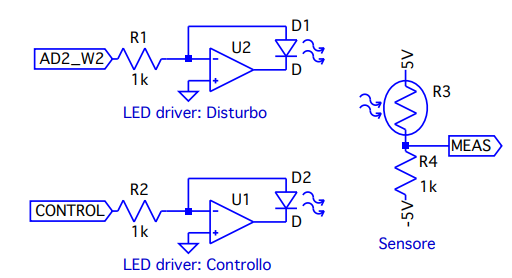
\includegraphics[scale=0.7]{noisegen}
    \caption{Schema dei circuiti di emissione e rilevazione di intensità
    luminosa.
    \label{schm: mesctrl}}
\end{figure}

\subsection{Analisi del funzionamento del circuito}
La fotoresistenza è una resistenza variabile in funzione dell'intensità
luminosa che incide su di essa. In particolare sappiamo che il valore di
resistenza $R_4$ e intensità della luce incidente sulla superficie della
fotoresistenza sono inversamente proporzionali.

Dalla formula del partitore di tensione sappiamo che il valore dell'uscita
\verb+MEAS+ dev'essere pari a
\begin{equation}
V\ped{MEAS} = (V_{CC} -  V_{EE})\frac{R_4}{R_4 + R_3} + V_{EE}
\end{equation}
Ci aspettiamo allora che aumentando la luce (quindi nel nostro caso pilotando
l'ingresso del LED driver di disturbo con una rampa), il valore di
$V\ped{MEAS}$ andrà ad aumentare sempre entro l'intervallo di tensioni
$(V_{EE}, V_{CC})$.

Riportiamo una serie di misure di $V\ped{MEAS}$ al variare del valore della
tensione continua generata all'ingresso \verb+W2+.
\begin{table}[htbp]
\centering
\begin{tabular}{@{}cc@{}}
\toprule
$V\ped{gen} \; [\si{\V}]$ & $V\ped{MEAS} \; [\si{\V}]$\\
\midrule
\midrule
$-4.2 \pm 0.3$ m 	& $ -4.99 \pm 0.05$	\\
$995 \pm 7$ m 	& $ -2.11 \pm 0.02 $	\\
$1.99 \pm 0.02$ 	& $ -1.01 \pm 0.08 $\\
$2.98 \pm 0.04$ 	& $ -359 \pm 3 $ m\\
$3.98 \pm 0.04$ 	& $ 42.1 \pm 0.7 $ m\\
$4.98 \pm 0.05$ 	& $ 335 \pm 3$ m\\
\bottomrule
\end{tabular}
\caption{Misure di $V\ped{MEAS}$ in funzione della tensione in ingresso nel
LED driver di disturbo}
\end{table}
Come ci aspettavamo il valore di $V\ped{meas}$ cresce all'aumentare
dell'intensità della luce incidente sulla fotoresistenza, cioè aumentando la
tensione in ingresso $V\ped{gen}$.

Per evidenziare meglio l'andamento del segnale in uscita dal partitore
\verb+MEAS+ al variare della tensione del segnale di disturbo si è
'automatizzata' la procedura inviando una rampa/gradinata discreta generata
da \verb+W2+ tramite script definito in Wavegen.
\begin{figure}[htbp]
    \centering
	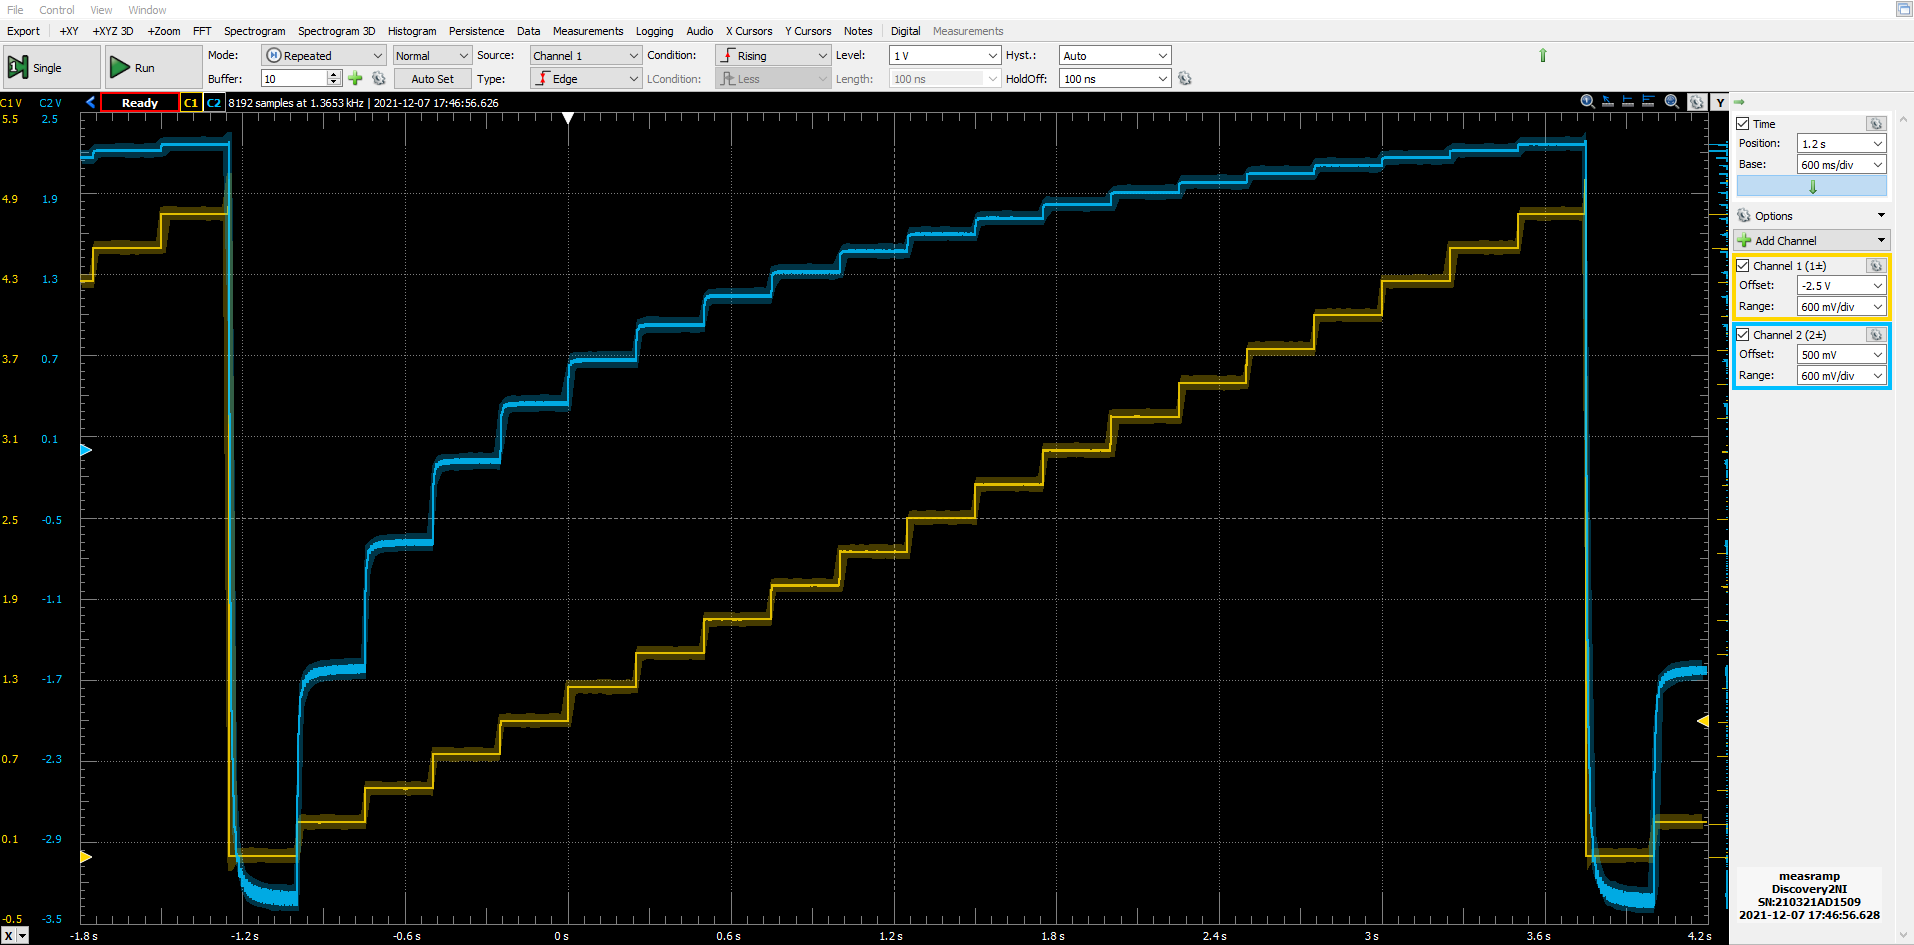
\includegraphics[width=\textwidth]{measgrad}
    \caption{Acquisizione presa dall'oscilloscopio dell'andamento nel tempo dei
	segnali in ingresso $W_2 (t)$ (CH1) e uscita $V\ped{MEAS} (t)$ (CH2)
	del partitore di tensione con \texttt{CONTROL} collegato a massa.
    \label{fig: measgrad}}
\end{figure}

%=======================
\section{Amplificatore di Noise rispetto a Set}
Si è costruito un amplificatore differenziale con guadagno $\sim 10$ a
partire dalle resistenze $R_5$, $R_6$ e $R_7$, $R_8$ secondo lo schema in
figura.
\begin{figure}[htbp]
    \centering
	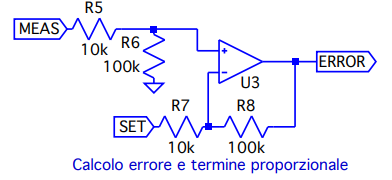
\includegraphics[scale=0.8]{errorgen}
    \caption{Schema circuitale dell'amplificatore differenziale realizzato
    \label{schm: errgen}}
\end{figure}
Lo scopo del circuito è quello di amplificare la differenza tra i segnali
$V\ped{SET}$ e $V\ped{MEAS}$ di un fattore 10.
Si è quindi misurato il guadagno per entrambi gli ingressi dell'OpAmp,
inviando un segnale a uno e collegando l'altro a massa. Ci si aspetta che nel
caso in cui SET sia collegato al segnale in ingresso, l'uscita dev'essere
invertita, mentre nel caso opposto MEAS e ERROR devono essere in fase.
\begin{figure}[htbp]
    \centering
	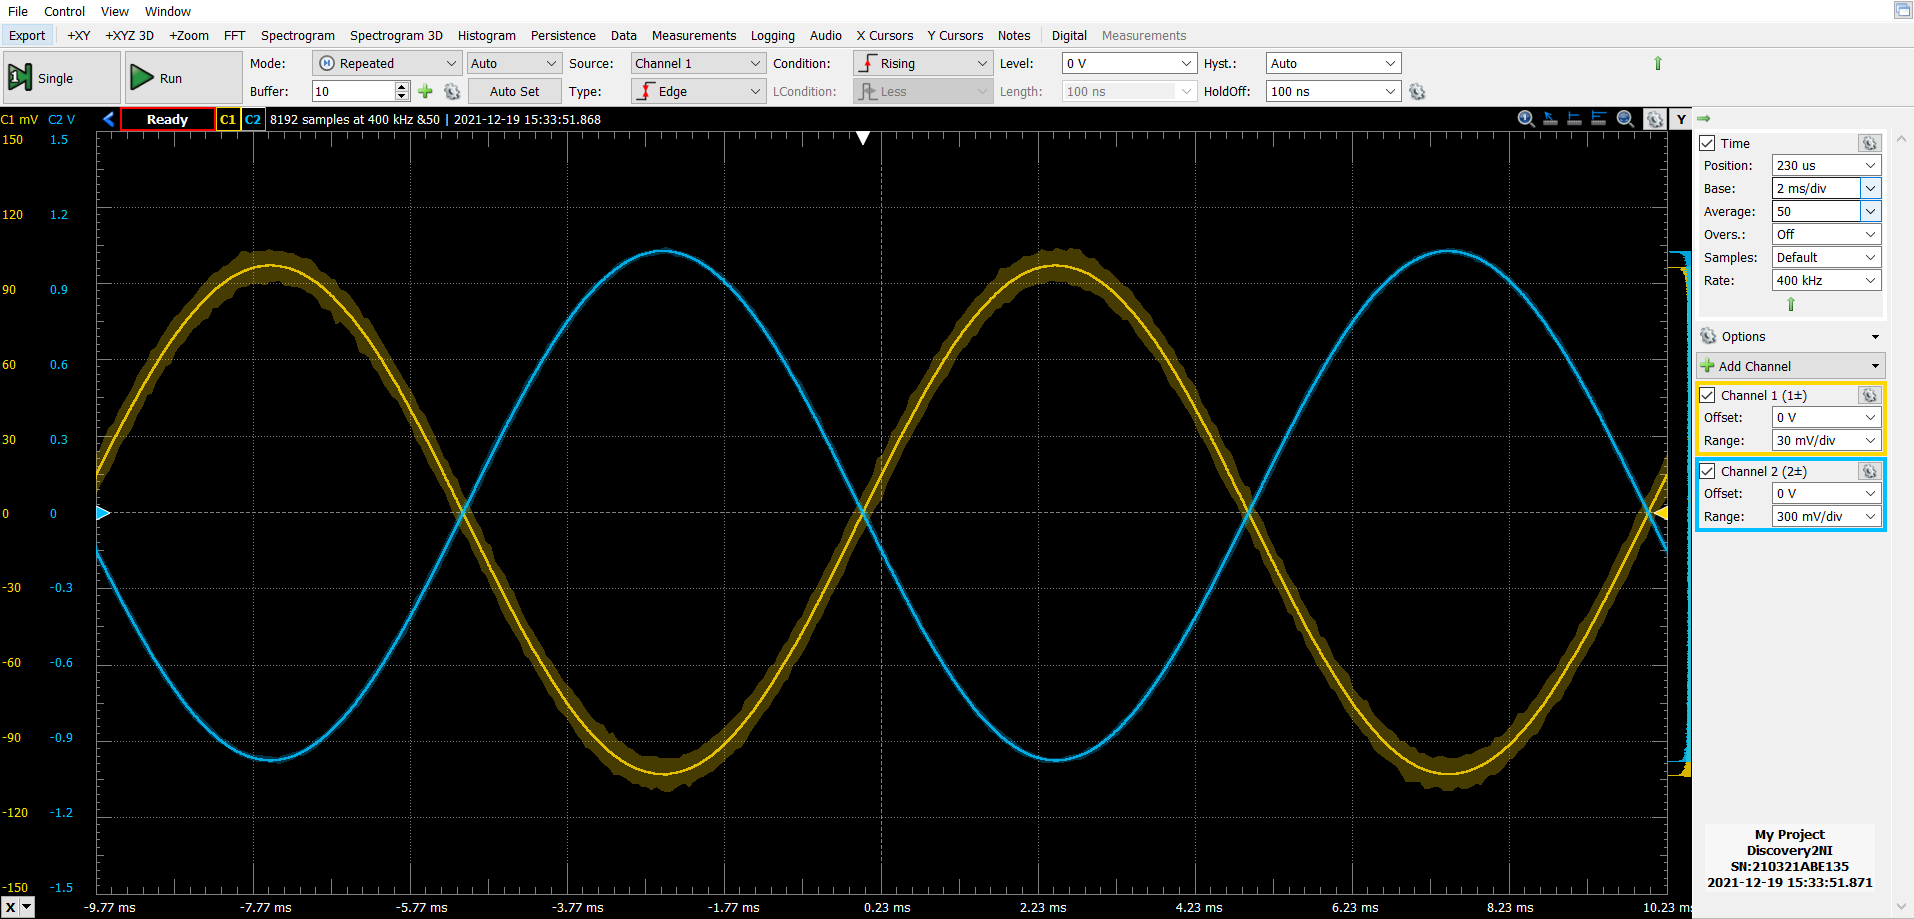
\includegraphics[width=\textwidth]{error.set}
    \caption{Acquisizione presa dall'oscilloscopio dell'andamento nel tempo dei
	segnali in ingresso $V\ped{SET} (t)$ (CH1) e uscita $V\ped{ERROR} (t)$ (CH2)
	dall'amplificatore differenziale con \texttt{MEAS} collegato a massa.
    \label{fig: errset}}
\end{figure}
\begin{figure}[htbp]
    \centering
	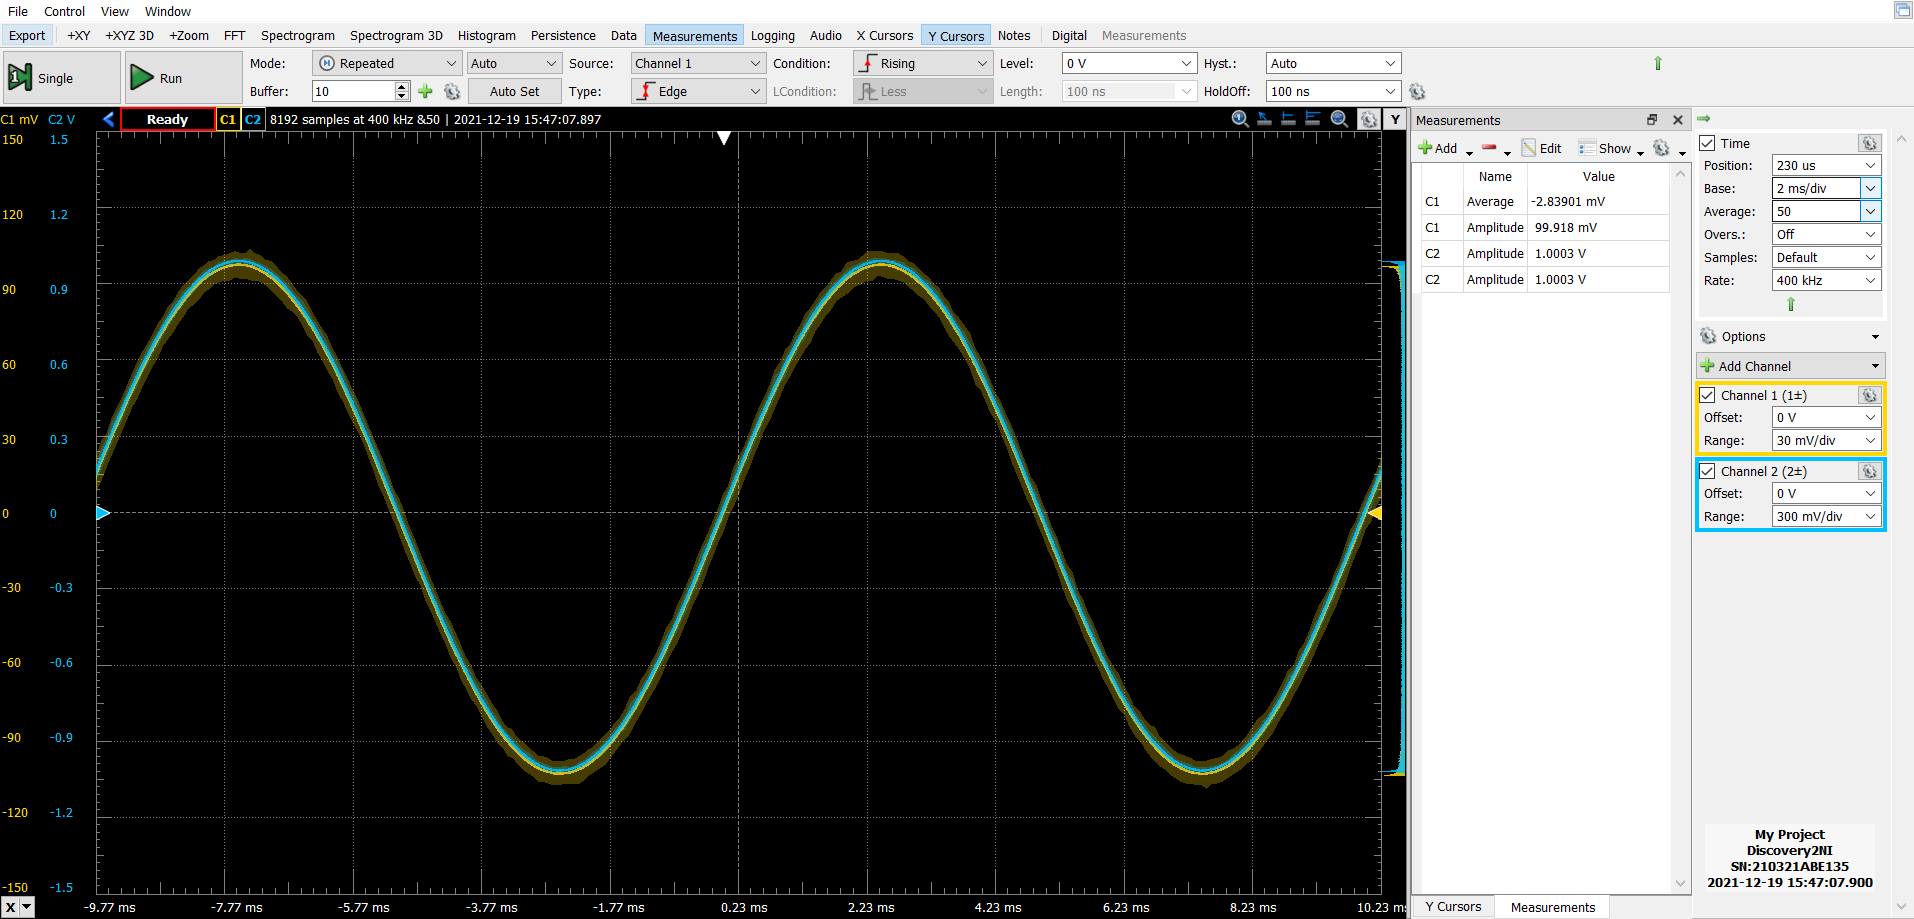
\includegraphics[width=\textwidth]{error.meas}
    \caption{Acquisizione presa dall'oscilloscopio dell'andamento nel tempo dei
	segnali in ingresso $V\ped{MEAS} (t)$ (CH1) e uscita $V\ped{ERROR} (t)$ (CH2)
	dall'amplificatore differenziale con \texttt{SET} collegato a massa.
    \label{fig: errmeas}}
\end{figure}

Abbiamo quindi misurato il guadagno per i due ingressi dell'OpAmp definito
come $A = \frac{V\ped{ERROR}}{V\ped{in}}$, da cui risulta
\begin{align*}
A\ped{SET} &= -10.01 \pm 0.14 \\
A\ped{MEAS} &= 10.01 \pm 0.14
\end{align*}

Per l'ingresso invertente \verb+SET+ e non-invertente \verb+MEAS+
rispettivamente, questi risultano compatibili con i valori di guadagno attesi
per l'amplificatore differenziale:
\begin{align*}
A\ped{SET} &= - \frac{R_8}{R_7} = -10.00 \pm 0.11 \\
A\ped{MEAS} &= \frac{R_6}{R_5} = 9.96 \pm 0.11
\end{align*}

Per controllare la tensione di riferimento si è poi costruito un circuito che
permettesse di variare $V\ped{SET}$ nello stesso intervallo
$(V_{EE}, V_{CC})$ attraverso l'uso di un potenziometro da
$R_{11} = 2 \si{k\ohm}$.
\begin{figure}[htbp]
    \centering
	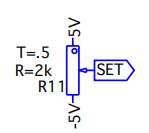
\includegraphics[scale=0.7]{setgen}
    \caption{Schema del circuito per la configurazione della tensione di
    riferimento.
    \label{schm: setgen}}
\end{figure}

Per verificare il corretto funzionamento del circuito amplificatore di
differenza tra i 2 segnali in ingresso, sappiamo che nel caso in cui
\verb+MEAS+ e \verb+SET+ siano uguali allora la differenza dev'essere nulla,
ovverosia in uscita dovremmo trovare $V\ped{ERROR} = 0$ V.
Difatti, collegando i terminali differenziali del CH1 dell'oscilloscopio
per misurare il segnale $V\ped{MEAS} (t)$ rispetto al segnale $V\ped{SET} (t)$
(registrando così la loro differenza) e CH2 per misurare $V\ped{ERROR} (t)$
all'uscita rispetto a massa troviamo che entrambi sono costanti e compatibili
con $\SI{0}{\V}$ come volevamo.
\begin{figure}[htbp]
    \centering
	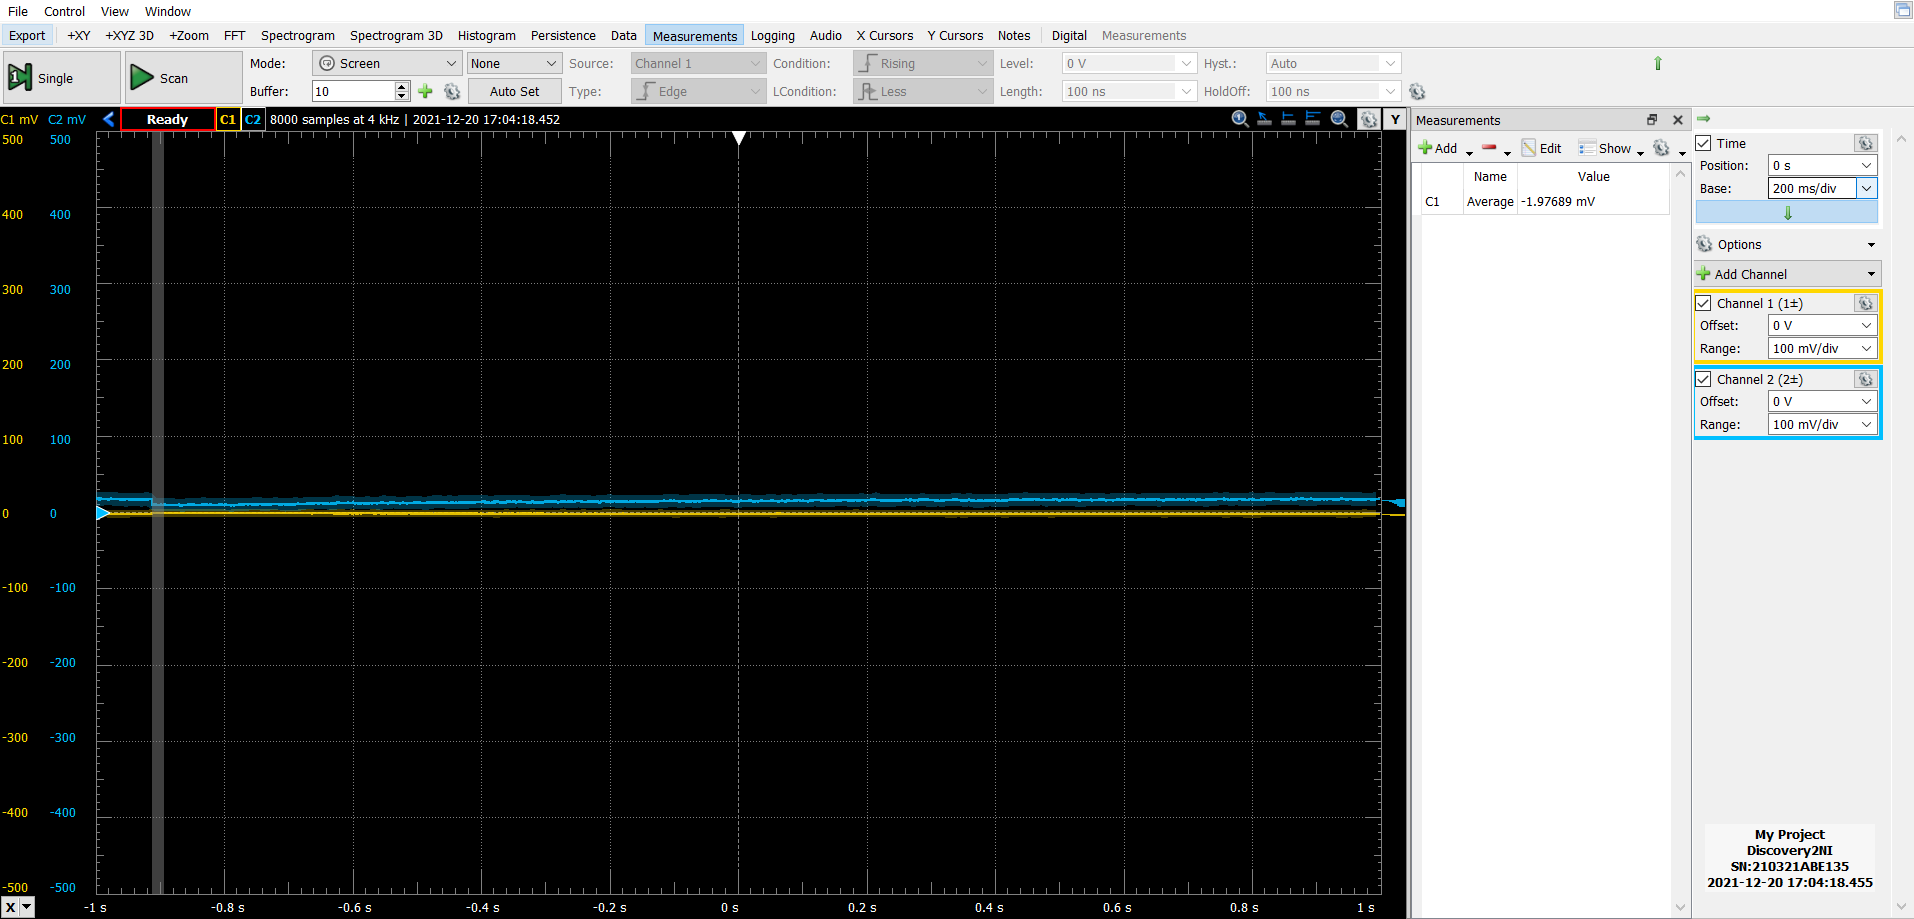
\includegraphics[width=\textwidth]{meas.same.set}
    \caption{Stampa a schermo dell'oscilloscopio nella condizione in cui le
    tensioni in \texttt{SET} e \texttt{MEAS} sono uguali. Con il canale uno
    si misura la differenza di potenziale tra $V\ped{MEAS}$ e $V\ped{SET}$,
    con il canale due invece $V\ped{ERROR}$ rispetto a massa.
    \label{fig: meas=set}}
\end{figure}

%=======================
\section{Controllo integrale}
Successivamente si è montato il circuito di controllo integrale, cioè un
circuito integratore RC costituito dalla resistenza $R_9$ del potenziometro e
da un condensatore $C_1$, montati secondo lo schema in \cref{fig: ctrlint}.
\begin{figure}[htbp]
    \centering
	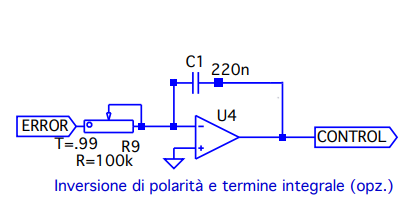
\includegraphics[scale=0.6]{controlgenint}
    \caption{schema circuitale del controllore ad azione integrale.
    \label{fig: ctrlint}}
\end{figure}

\section{Verifica del funzionamento del circuito}
Abbiamo collegato l'uscita \verb+CONTROL+ al driver per la luce di
controllo e l'uscita del circuito di generazione errore all'entrata del
circuito di controllo integrale.
A questo punto è stato sufficiente passivare il generatore di luce di
disturbo e spostare il contatto strisciante di $R_9 = 100 \; \si{k\ohm}$ a
fine corsa per poter osservare l'accensione del LED di controllo.

Si nota immediatamente come la risposta del LED di controllo sia estremamente
sensibile alla quantità di luce che incide sulla fotoresistenza. Per questo
motivo abbiamo scelto di coprire il circuito e spostarci quanto meno possibile
durante le prese dati, al fine di schermare l'apparato sperimentale da
eventuali sorgenti di disturbo casuali (e.g. persone/cose che si spostano
in prossimità della fotoresistenza).

Si è riusciti a verificare la risposta del circuito con LED di controllo ad un
intervento esterno di riduzione della luce: si sono interposte delle buste di
plastica trasparenti tra il diodo e la fotoresistenza, dunque abbiamo
osservato il LED aumentare l'intensità luminosa in uscita di conseguenza.

\section{Risposta ad un'onda quadra}\label{sec: intsqwresp}
Si è quindi passati allo studio della risposta del circuito ad una luce di
disturbo, in questo primo caso pilotata da un'onda quadra.
Per prima cosa occorre fissare un valore di tensione di riferimento \verb+SET+:
si è scelta come intensità luminosa arbitraria quella che \verb+MEAS+ legge
quando uno dei 2 driver LED è pilotato con una tensione di $\SI{1}{\V}$.
Infine si è impostato il valore di resistenza del potenziometro $R_{11}$ in
modo tale che \verb+MEAS+ e \verb+SET+ si trovassero alla stessa tensione.

A questo punto si è inviata al LED driver di disturbo un'onda quadra compresa
tra $0$ e $150 \; \si{m\V}$ con frequenza pari a $f = 1 \si{\Hz}$.
Osservando l'andamento nel tempo dei segnali $V\ped{CONTROL} (t)$ e
$V\ped{MEAS} (t)$ si riesce ad apprezzare il comportamento del circuito sotto
studio; questo cerca di ``correggere'' il disturbo esterno al fine di
mantenere il valore dell'osservabile $V\ped{MEAS}$ costante nel tempo.
Infatti il segnale in \verb+CONTROL+ è un'onda quadra in opposizione di fase
a quella di disturbo ma con difetti di \emph{overshoot}, dovuti al tempo
caratteristico di risposta del circuito integratore alla variazione rapida
nei fronti di discesa e salita dell'onda quadra $W_2 (t)$.
\begin{figure}[htbp]
    \centering
	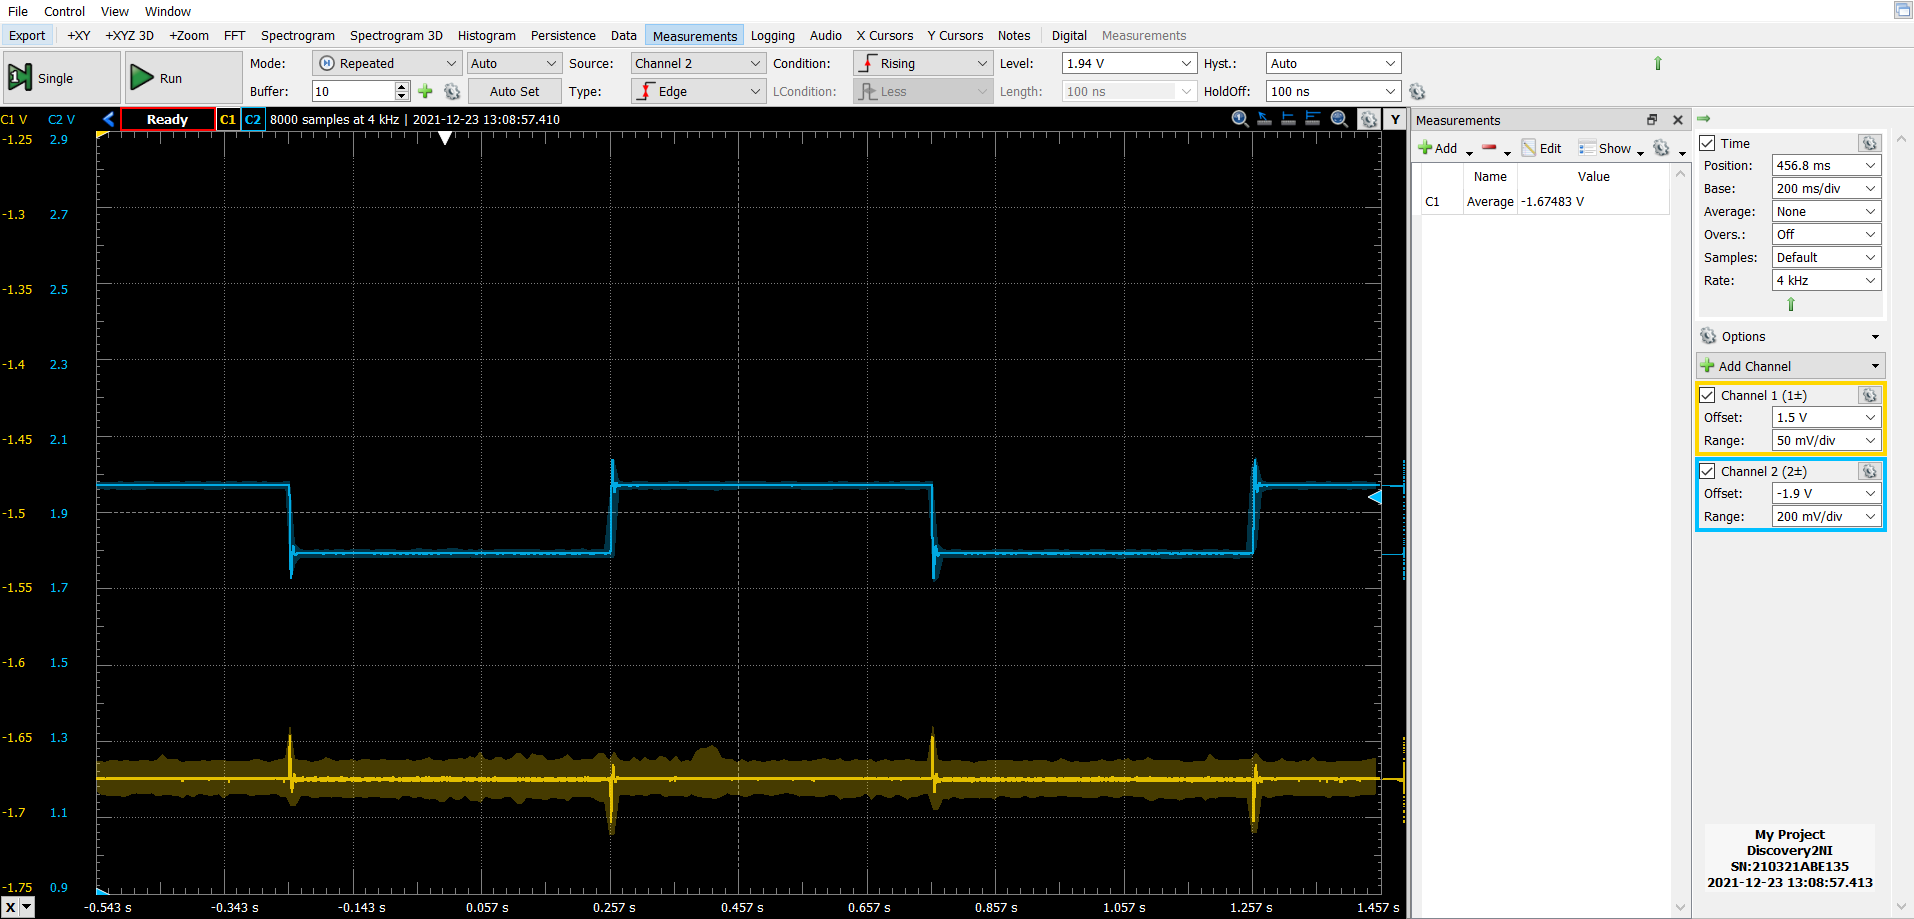
\includegraphics[width=\textwidth]{control7.meas}
    \caption{Acquisizione all'oscilloscopio dell'andamento nel tempo dei
    segnali in \texttt{MEAS} (CH1) e di \texttt{CONTROL} (CH2) rispetto a
    massa.
    \label{fig: ctrlmeas}}
\end{figure}
\begin{figure}[htbp]
    \centering
	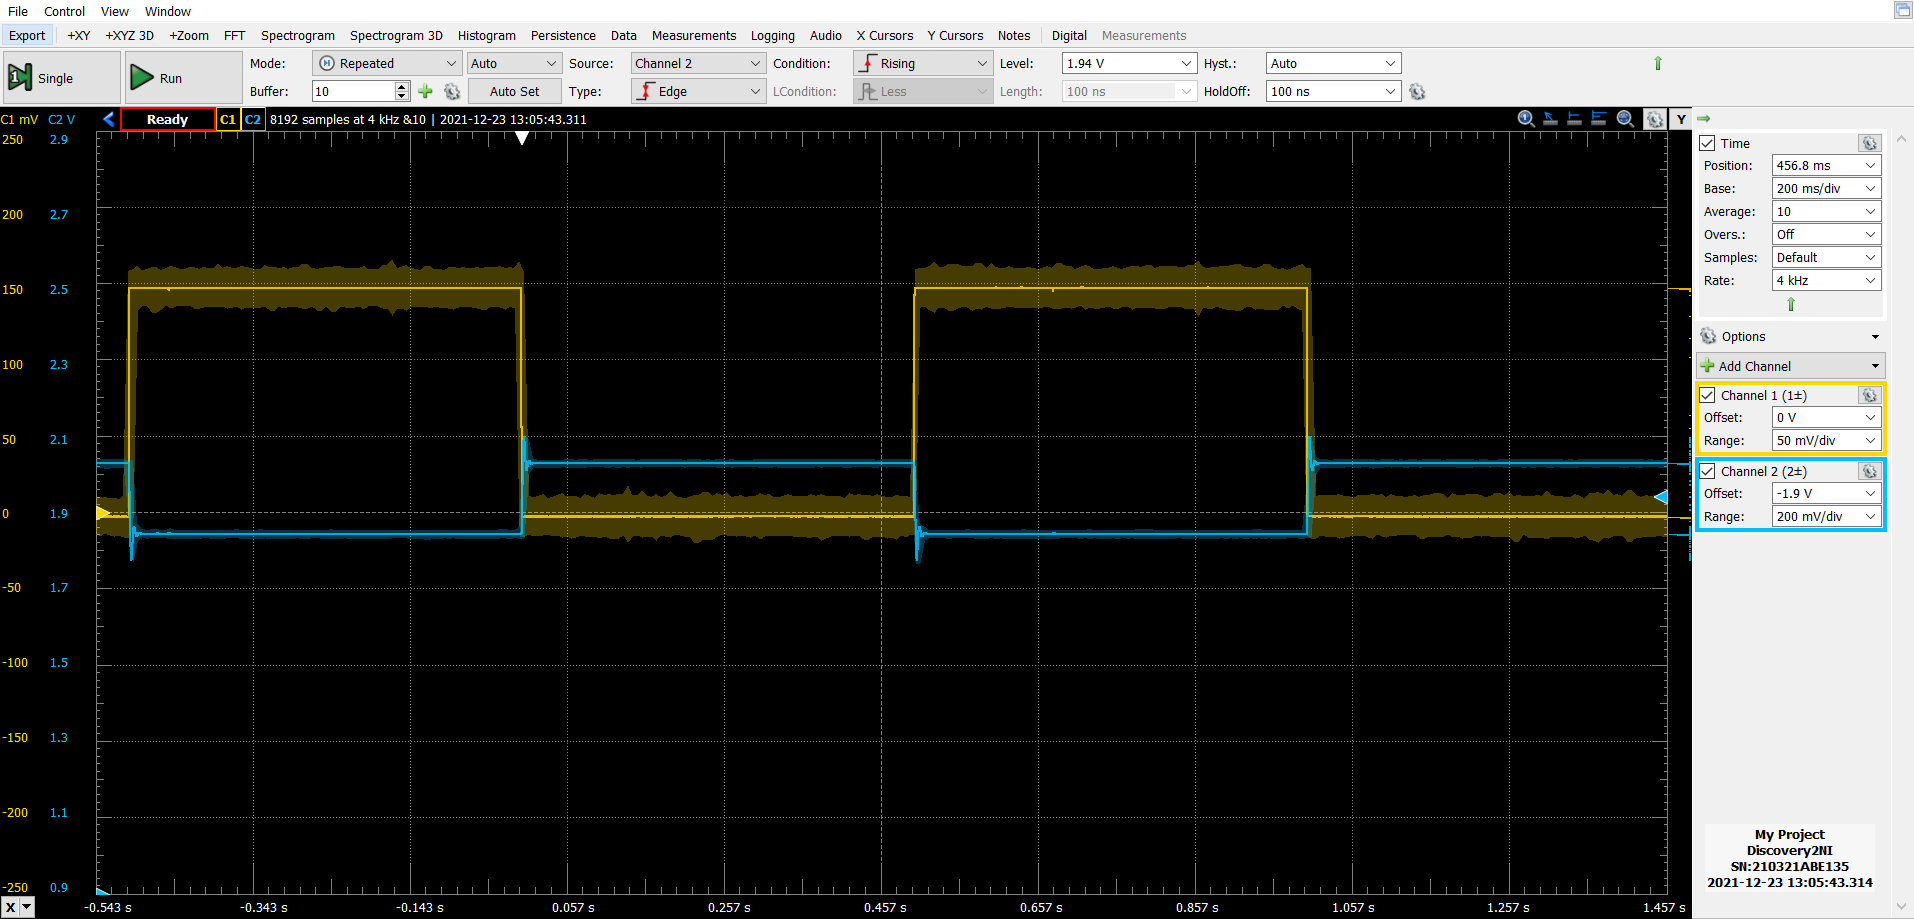
\includegraphics[width=\textwidth]{control7}
    \caption{Acquisizione all'oscilloscopio dei segnali $W_2 (t)$
    (CH1) e dell'onda pilota del LED di disturbo $V\ped{CONTROL} (t)$ (CH2).
    \label{fig: ctrlnoise}}
\end{figure}

Dunque abbiamo osservato il comportamento del segnale in \verb+error+ al
variare della resistenza del potenziometro $R_9$. Si nota che anche questo
segnale ha un andamento `inversamente' proporzionale all'onda quadra di
disturbo, cioè rimane costante a $0$ V durante i periodi alti e bassi, mentre
in corrispondenza dei fronti di discesa e salita di $W_2 (t)$ assume la forma
di un'oscillazione smorzata esponenzialmente. Per essere più precisi
$V\ped{ERROR} (t)$ ha sempre la forma di una serie di oscillazioni smorzate di
segno alternante che si ripetono ogni semi-periodo dell'onda quadra in
\verb+NOISE+, ma al variare della posizione del trimmer cambiano sensibilmente
l'ampiezza iniziale, la frequenza e il tempo di smorzamento $\tau$ dopo cui
l'uscita dell'amplificatore differenziale torna ad essere nulla, una volta che
l'oscillazione si è spenta.
\begin{figure}[htbp]
    \centering
	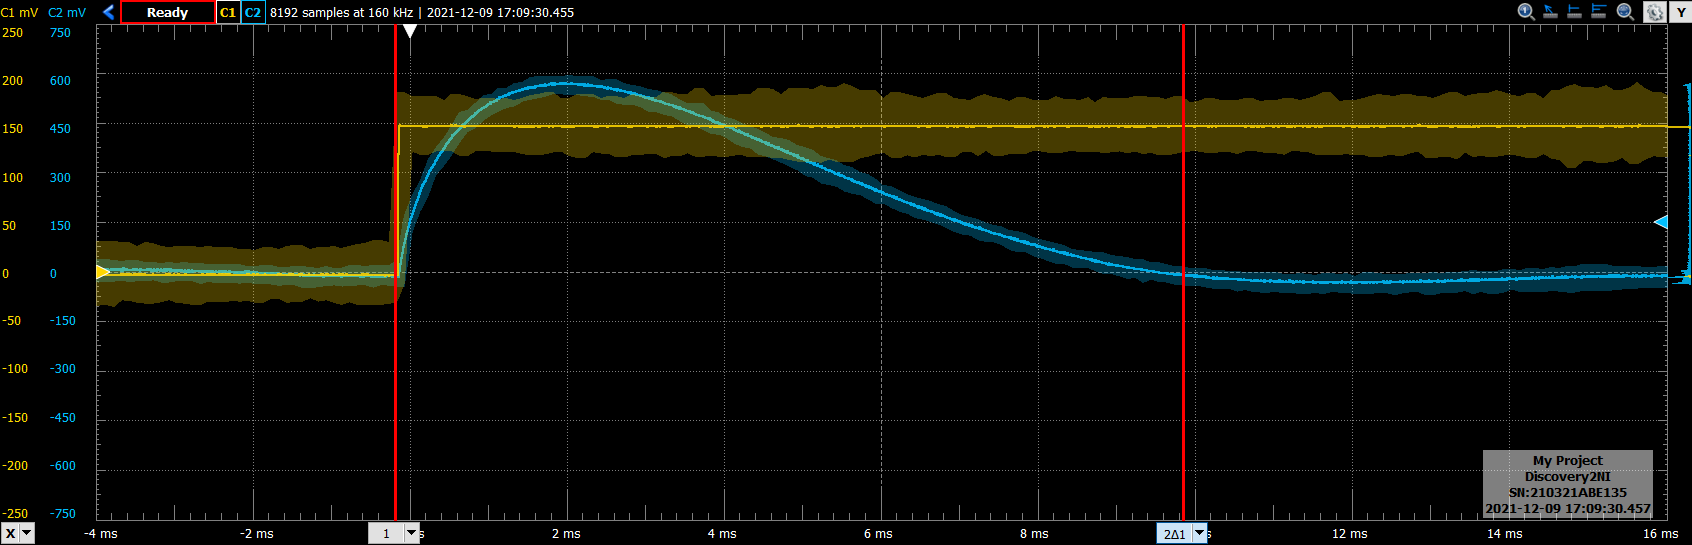
\includegraphics[width=\textwidth]{7}
    \caption{Acquisizione presa dall'oscilloscopio dell'andamento del segnale
    $V\ped{ERROR} (t)$ (CH2) rispetto all'onda quadra $W_2 (t)$ di disturbo
    (CH1).
    \label{fig: errnoise}}
\end{figure}

Tramite cursori si è quindi misurato il tempo di smorzamento
dell'oscillazione/`overshoot' in \verb+ERROR+ e lo abbiamo confrontato con il
tempo caratteristico di risposta del circuito integratore definito da
$\tau\ped{RC} = R_9 C_1$.
\begin{table}[htbp]
\centering
\begin{tabular}{@{}lll@{}}
\toprule
Resistenza $R_9$ $[\si{k\ohm}]$ & $\tau$ [ms] & $\tau\ped{RC}$ [ms] \\
\midrule
\midrule
$103.4 \pm 0.8 $ & $20.7 \pm 0.4$ & $ 21.4 \pm 0.9$ \\
$92.8 \pm 0.8$	& $19.0 \pm 0.3$ & $ 19.2 \pm 0.8 $ \\
$67.7 \pm 0.6$	& $15.3 \pm 0.3$ & $ 14.0 \pm 0.6 $ \\
$40.2 \pm 0.4$	& $8.2 \pm 0.2$ & $ 8.6 \pm 0.3 $ \\
$26.4 \pm 0.3$	& $5.8 \pm 0.1$ & $ 5.6 \pm 0.2 $ \\
$11.98 \pm 0.10$ & $2.72 \pm 0.10$ & $2.5 \pm 0.1$ \\
\\
$7.34 \pm 0.06$ & $3.24 \pm 0.10$ & $ 1.52 \pm 0.06$ \\
$2.78 \pm 0.03$ & $0.92 \pm 0.05$ & $ 0.59 \pm 0.02$ \\
\bottomrule
\end{tabular}
\caption{Misura dei tempi di smorzamento delle oscillazioni
di $V\ped{ERROR} (t)$ e confronto con tempo caratteristico di risposta
dell'integratore al variare di $R_9$.}
\end{table}

Da cui vediamo che le prime misure di tempo risultano compatibili con i loro
valori attesi, mentre per valori di resistenza $R_9 < \SI{10}{k\ohm}$ queste
tendono a discostarvisi sempre di più al diminuire del valore di resistenza.
Risulta difficile da valutare se questa deviazione sia dovuta ad accoppiamenti
capacitivi fra basetta, fili e componenti passivi del circuito, alle capacità
parassite dentro il TL081 o ad entrambi, che non stiamo considerando nel
nostro modello.

Per evidenziare ancora meglio l'effetto che la diminuzione della resistenza
del potenziometro $R_9$ (quindi dello smorzamento/dissipazione) e il
conseguente aumento del guadagno del controllore integrale hanno sul transiente
in \verb+ERROR+ se ne riporta in \cref{fig: intR9osc} la sovrapposizione degli
andamenti nel tempo osservati dall'oscilloscopio
\begin{figure}[htbp]
    \centering
	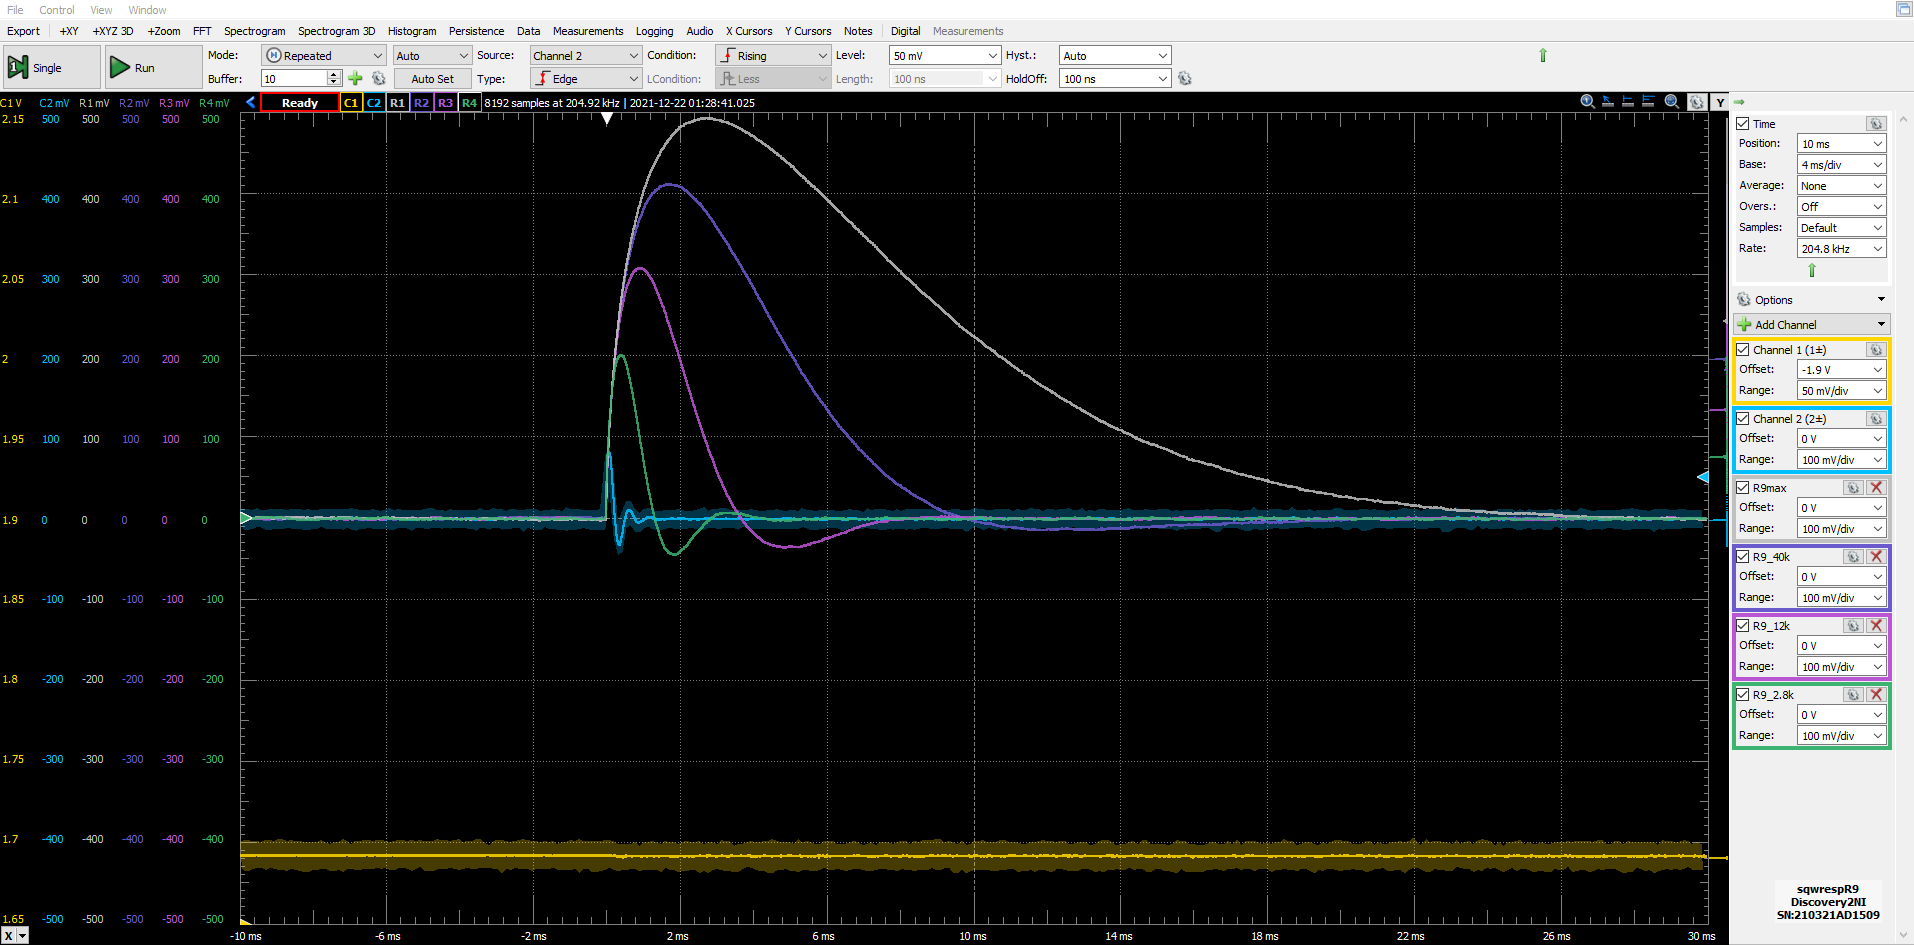
\includegraphics[width=\textwidth]{sqwrespfunction}
    \caption{Acquisizione all'oscilloscopio della modifica del segnale
    $V\ped{ERROR} (t)$ (CH2) al variare della resistenza del potenziometro
    $R_9$. In ordine di ampiezza iniziale decrescente per $R_9 =
    (103.0 \pm 0.6 \; \si{k\ohm})$, $(40.2 \pm 0.4 \; \si{k\ohm})$,
    $(11.98 \pm 0.10 \; \si{k\ohm})$, $(2.78 \pm 0.03 \; \si{k\ohm})$ e
    $(197 \pm 2 \; \si{\ohm})$.
    In giallo la risposta costante dell'osservabile in \texttt{MEAS} su (CH1).
    \label{fig: intR9osc}}
\end{figure}
Da cui vediamo come l'oscillazione prima che il sistema e $V\ped{ERROR} (t)$
tornino a regime è inizialmente sovrasmorzata ed è sempre più debolmente
smorzata, decrescente in ampiezza e di frequenza crescente al diminuire della
resistenza $R_9$. Questo è compatibile con quanto ci aspettiamo dalla funzione
di trasferimento del controllore, per cui ad una diminuzione del tempo di
risposta dell'azione integrale corrisponde un aumento della frequenza e del
tempo di smorzamento del transitorio dopo la risposta ad un gradino di
tensione, cioè ad una riduzione del margine di stabilità del sistema.

\section{Risposta ad una rampa}
Come prima si è reimpostato il valore della resistenza del potenziometro al
massimo ($100 \; \si{k\ohm}$ nominali) ma stavolta si è pilotato il driver LED
di disturbo con un'onda triangolare compresa tra $0$ e $150 \si{m\V}$ di
frequenza $f = 10 \; \si{\Hz}$ e duty-cycle $\text{dc} = (10 \percent$),
($90 \percent$). Ne riportiamo la risposta osservata in \verb+ERROR+ come
campionata dall'oscilloscopio per i due valori di duty-cycle in
\cref{fig: erramp10} e \cref{fig: erramp90}.
\begin{figure}[htbp]
    \centering
	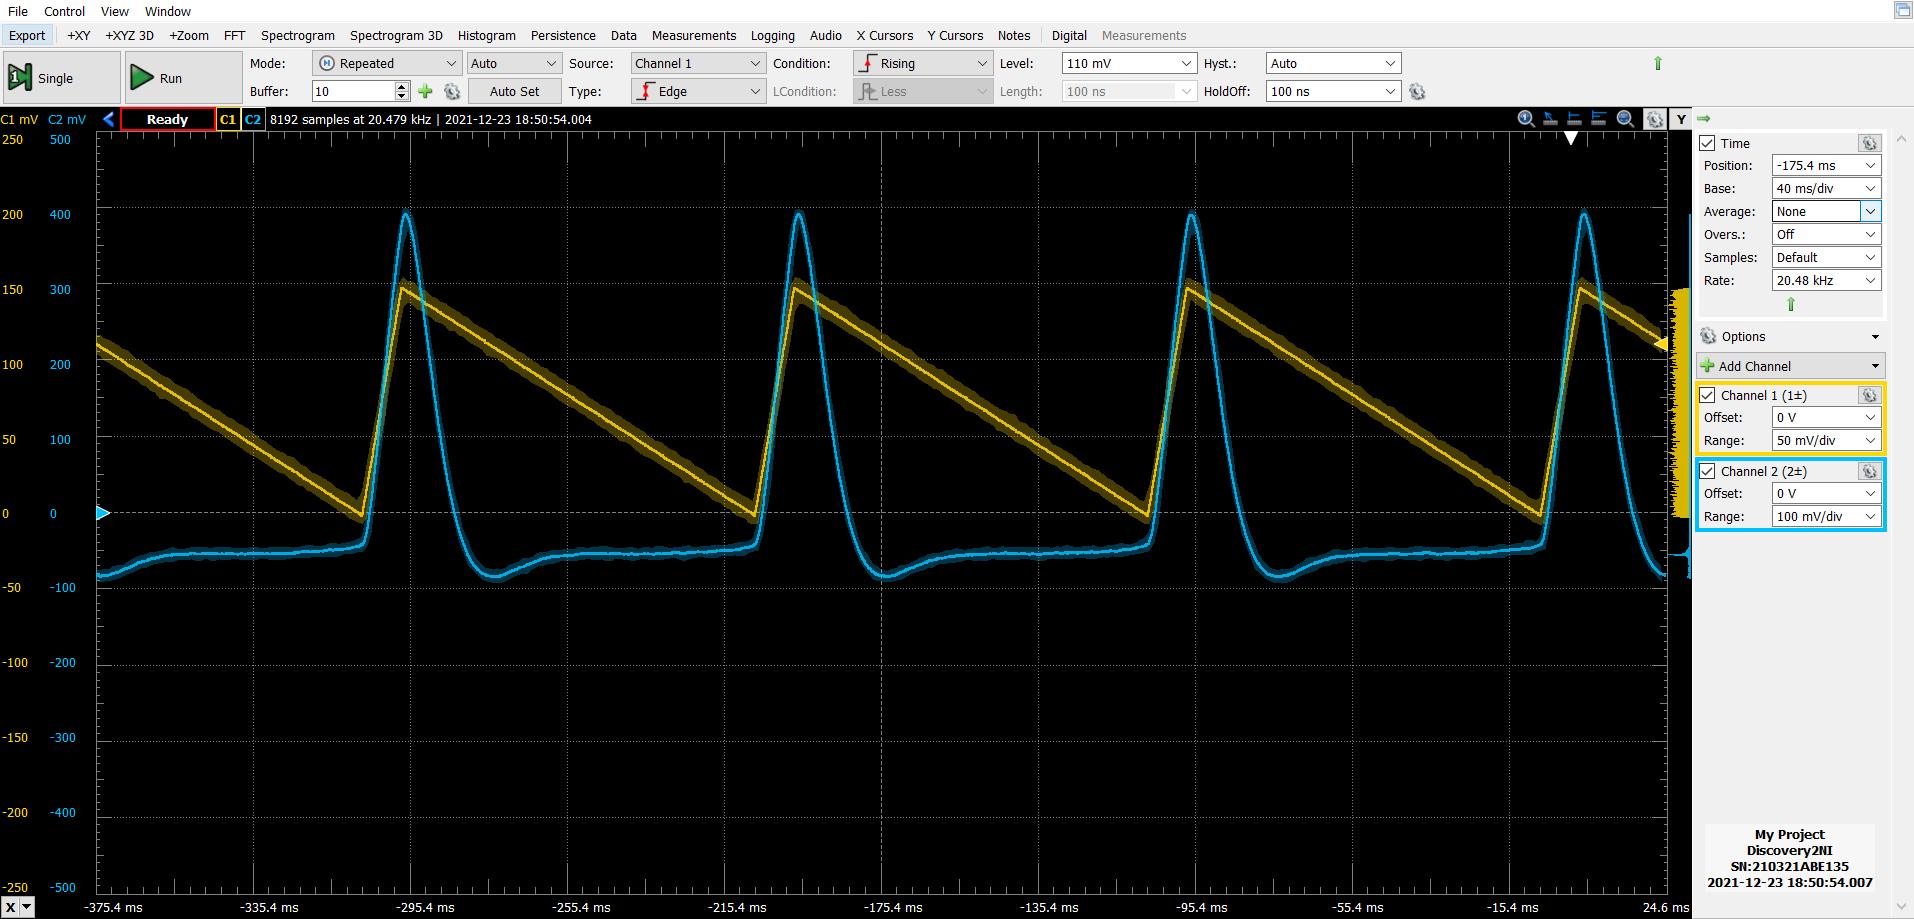
\includegraphics[width=\textwidth]{8}
    \caption{Acquisizione dall'oscilloscopio degli andamenti nel tempo dei
    segnali in \texttt{ERROR} (CH2) e del segnale di disturbo $W_2 (t)$ (CH1)
    con l'onda triangolare di duty-cycle $10 \percent$
    \label{fig: erramp10}}
\end{figure}
\begin{figure}[htbp]
    \centering
	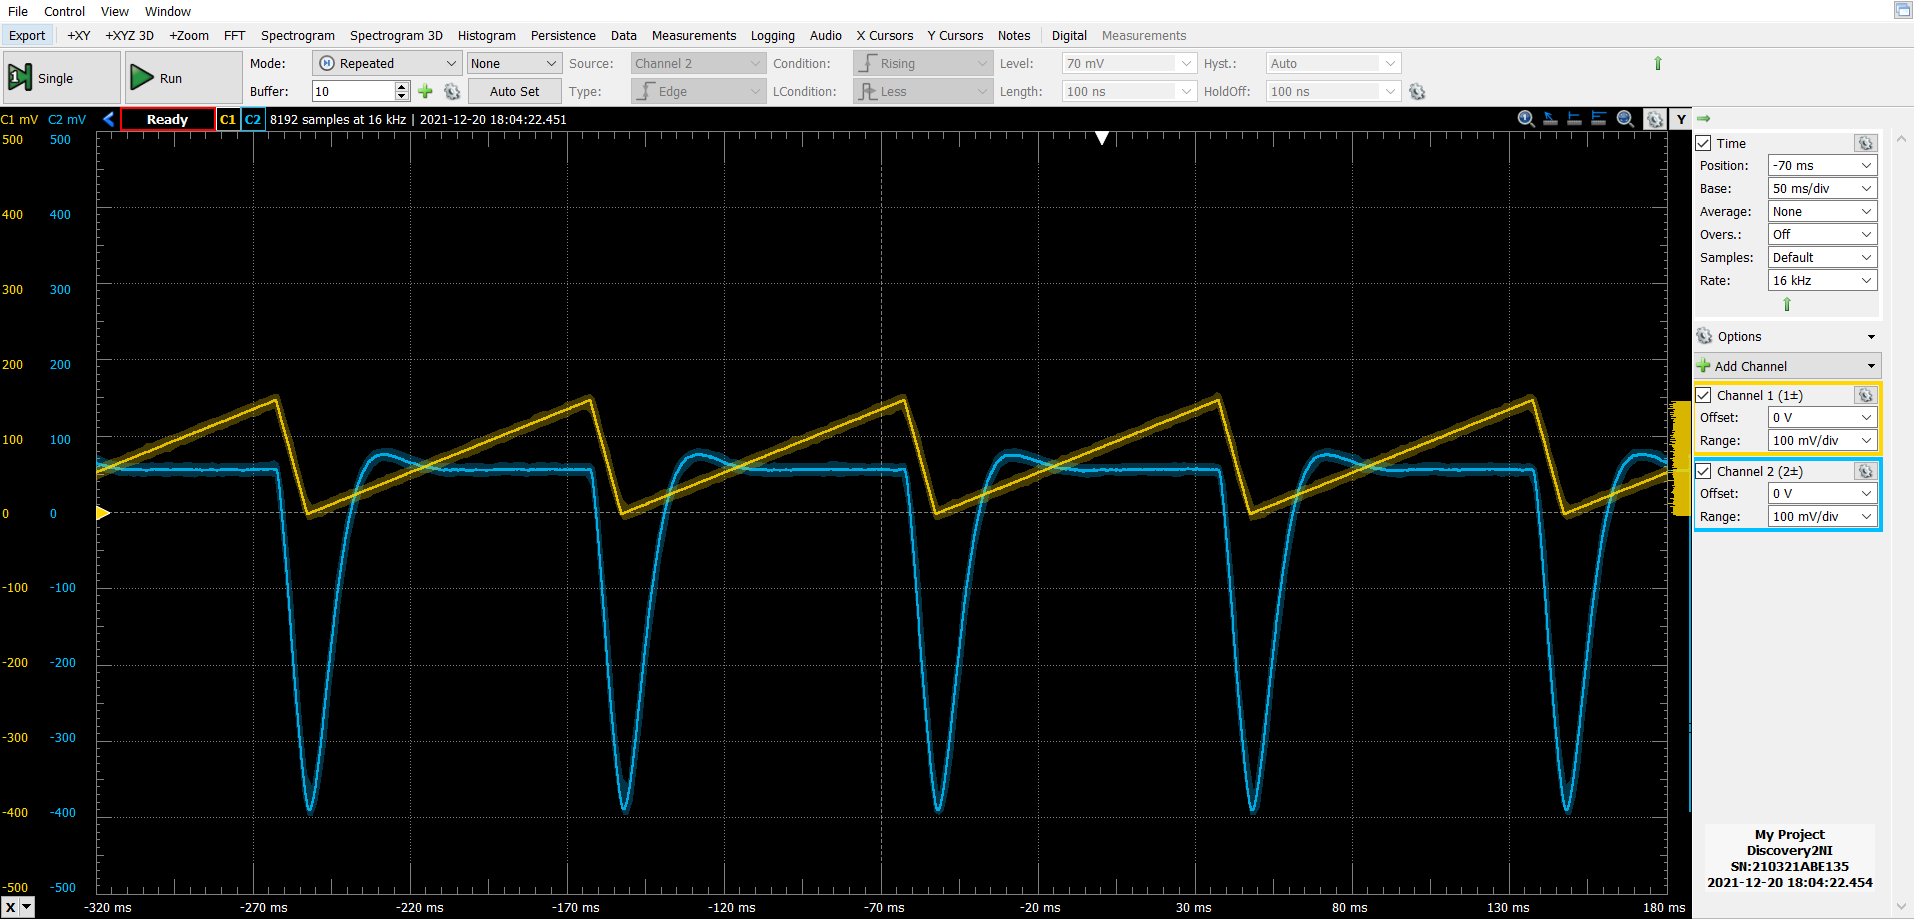
\includegraphics[width=\textwidth]{8.1}
    \caption{Acquisizione dall'oscilloscopio degli andamenti nel tempo dei
    segnali in \texttt{ERROR} (CH2) e del segnale di disturbo $W_2 (t)$ (CH1)
    con l'onda triangolare di duty-cycle $10 \percent$.
    \label{fig: erramp90}}
\end{figure}

Anche in questo caso il circuito di amplificazione dell'errore si comporta
in maniera simile ad un derivatore. Questo è ragionevole, dal momento che il
segnale di controllo dev'essere proporzionale all'integrale del
segnale di errore, e per poter bilanciare il disturbo luminoso in \verb+NOISE+,
l'uscita del circuito di controllo dev'essere un'onda triangolare in
opposizione di fase a quella con cui pilotiamo il LED di disturbo; dunque
l'ingresso \verb+ERROR+ del regolatore dev'essere proporzionale alla derivata
del segnale all'uscita \verb+CONTROL+.

In corrispondenza del fronte ripido della rampa di disturbo asimmetrica
$W_2 (t)$, in $V\ped{ERROR} (t)$ troviamo una serie di picchi smorzati
simili ai transienti osservati prima nella risposta ad un'onda quadra
in \cref{sec: intsqwresp} dovuti al tempo finito di risposta del controllore
ad azione integrale.
In effetti possiamo considerare il fronte ripido del segnale di disturbo come
il fronte di salita di un gradino come prima, solo con un tempo di salita
molto più lungo\footnote{Mentre prima avevamo come tempo di salita
$t\ap{sqw}\ped{rise} \approx 20 \; \si{n\s}$ per l'onda triangolare abbiamo
misurato $t\ap{trg}\ped{rise} = 10.0 \pm 0.4 \; \si{m\s}$, che differiscono
di quasi 6 ordini di grandezza.} di quello caratteristico dell'onda quadra
generata dall'AD2.

Sempre per via del fatto che il circuito integratore reagisce in un tempo
finito (dell'ordine di $\tau_{RC} = R_9 C_1$) in risposta a dei cambiamenti
di $V\ped{MEAS} (t)$ rispetto a $V\ped{SET}$, il segnale di errore non potrà
mai essere nullo. Infatti se lo fosse il controllore non attuerebbe alcun
cambiamento, e questo dovrebbe avvenire solamente nel caso in cui si abbia
una fonte di disturbo luminosa in \verb+NOISE+ costante nel tempo.

\section{Risposta in frequenza}
Si è misurata la funzione di trasferimento tra il generatore di disturbo e
il segnale di errore per diverse posizioni del contatto strisciante del
potenziometro $R_9$ per cui il sistema ha il funzionamento atteso tramite
lo strumento Network dell'AD2.
In particolare si è inviato come segnale in ingresso (\verb+NOISE+) una
sinusoide di frequenza compresa tra $\SI{1}{\Hz}$ e $\SI{1}{k\Hz}$ di
ampiezza costante pari a $100 \; \si{m\V}$ e offset di $50 \; \si{m\V}$
e si è registrata la risposta in frequenza del sistema monitorandone l'uscita
in \verb+ERROR+.
\begin{figure}[htbp]
    \centering
	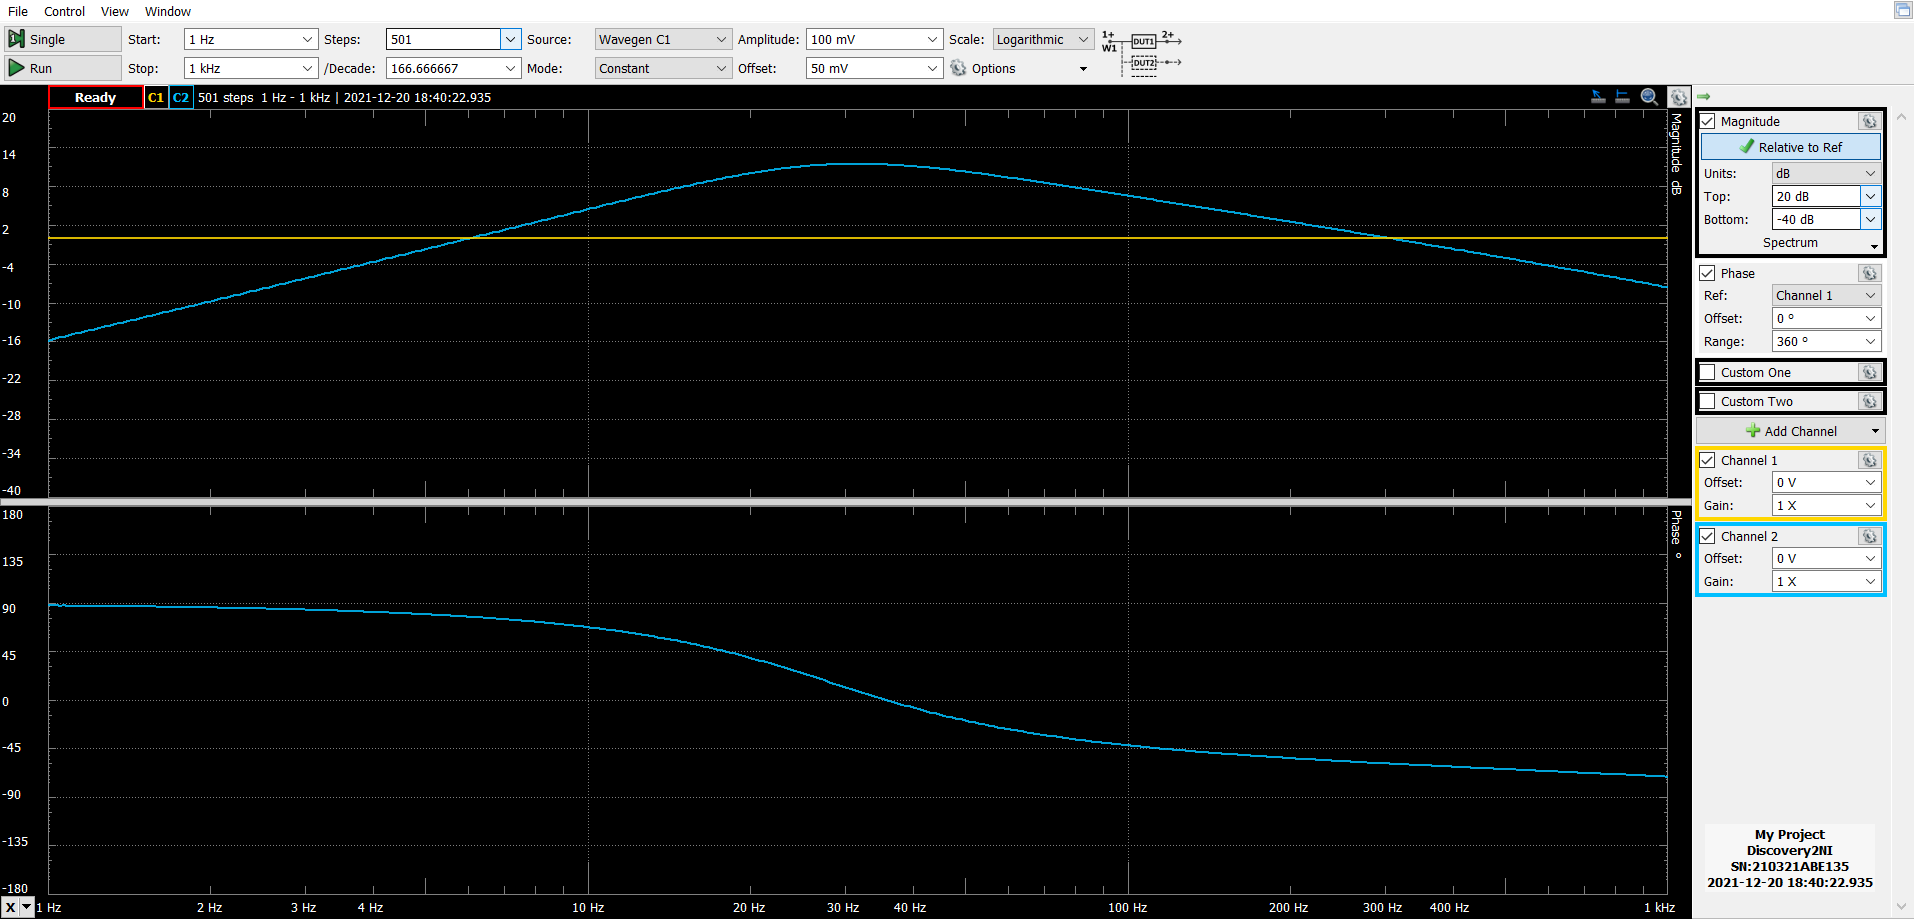
\includegraphics[width=\textwidth]{103.4k}
    \caption{Plot di Bode ottenuto dallo scan con Network tra $\SI{1}{\Hz}$ e
	$\SI{1}{k\Hz}$ con un segnale sinusoidale in ingresso al LED di disturbo di
	ampiezza $v\ped{in} = \SI{100}{m\V}$ e offset costante di $\SI{50}{m\V}$.
	In azzurro la risposta in frequenza del segnale in \texttt{ERROR} per un
	valore di resistenza del potenziometro $R_9 = 103.4 \pm 0.8 \; \si{k\ohm}$.
    \label{fig: netR103}}
\end{figure}
\begin{figure}[htbp]
    \centering
	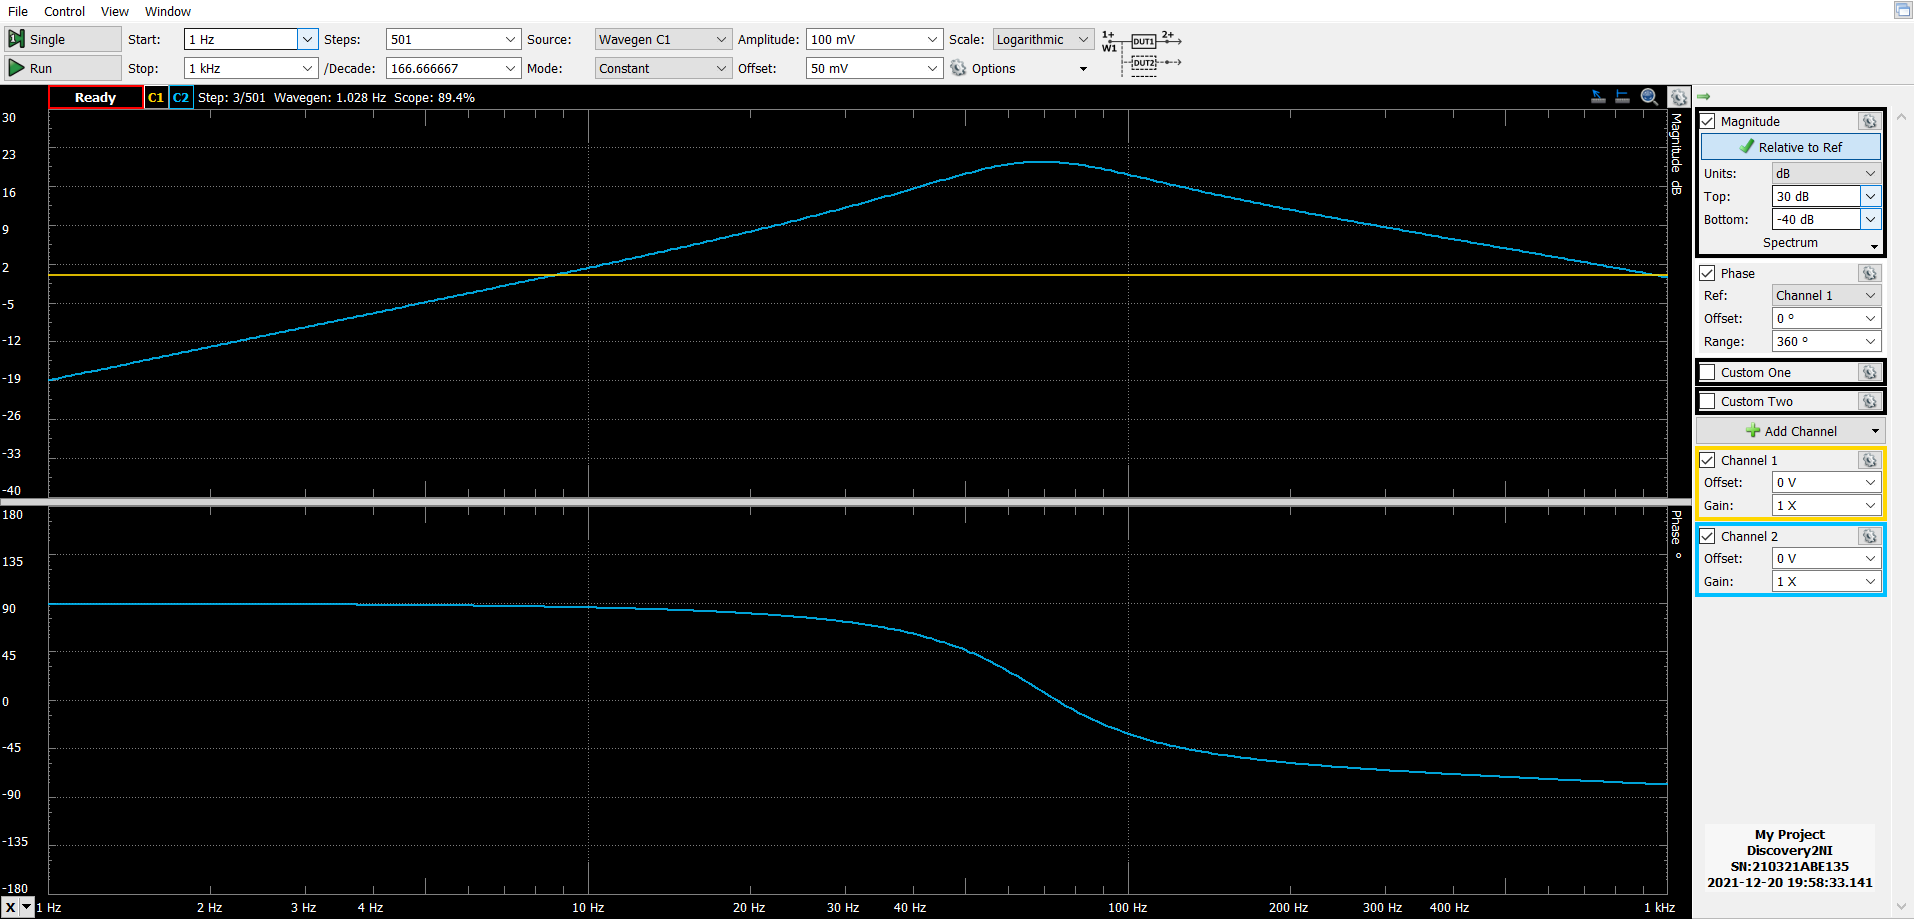
\includegraphics[width=\textwidth]{76.1k}
    \caption{Plot di Bode ottenuto dallo scan con Network tra $\SI{1}{\Hz}$ e
	$\SI{1}{k\Hz}$ con un segnale sinusoidale in ingresso al LED di disturbo di
	ampiezza $v\ped{in} = \SI{100}{m\V}$ e offset costante di $\SI{50}{m\V}$.
	In azzurro la risposta in frequenza del segnale in \texttt{ERROR} per un
	valore di resistenza del potenziometro $R_9 = 76.1 \pm 0.6 \; \si{k\ohm}$.
    \label{fig: netR76}}
\end{figure}

Per riuscire a evidenziare meglio come si modifica al variare di $R_9$ la
risposta in frequenza del circuito riportiamo in un unico grafico la
sovrapposizione di alcuni scan di Network condotti alla stessa maniera dei
primi due in \cref{fig: netR9func}.
\begin{figure}[htbp]
    \centering
	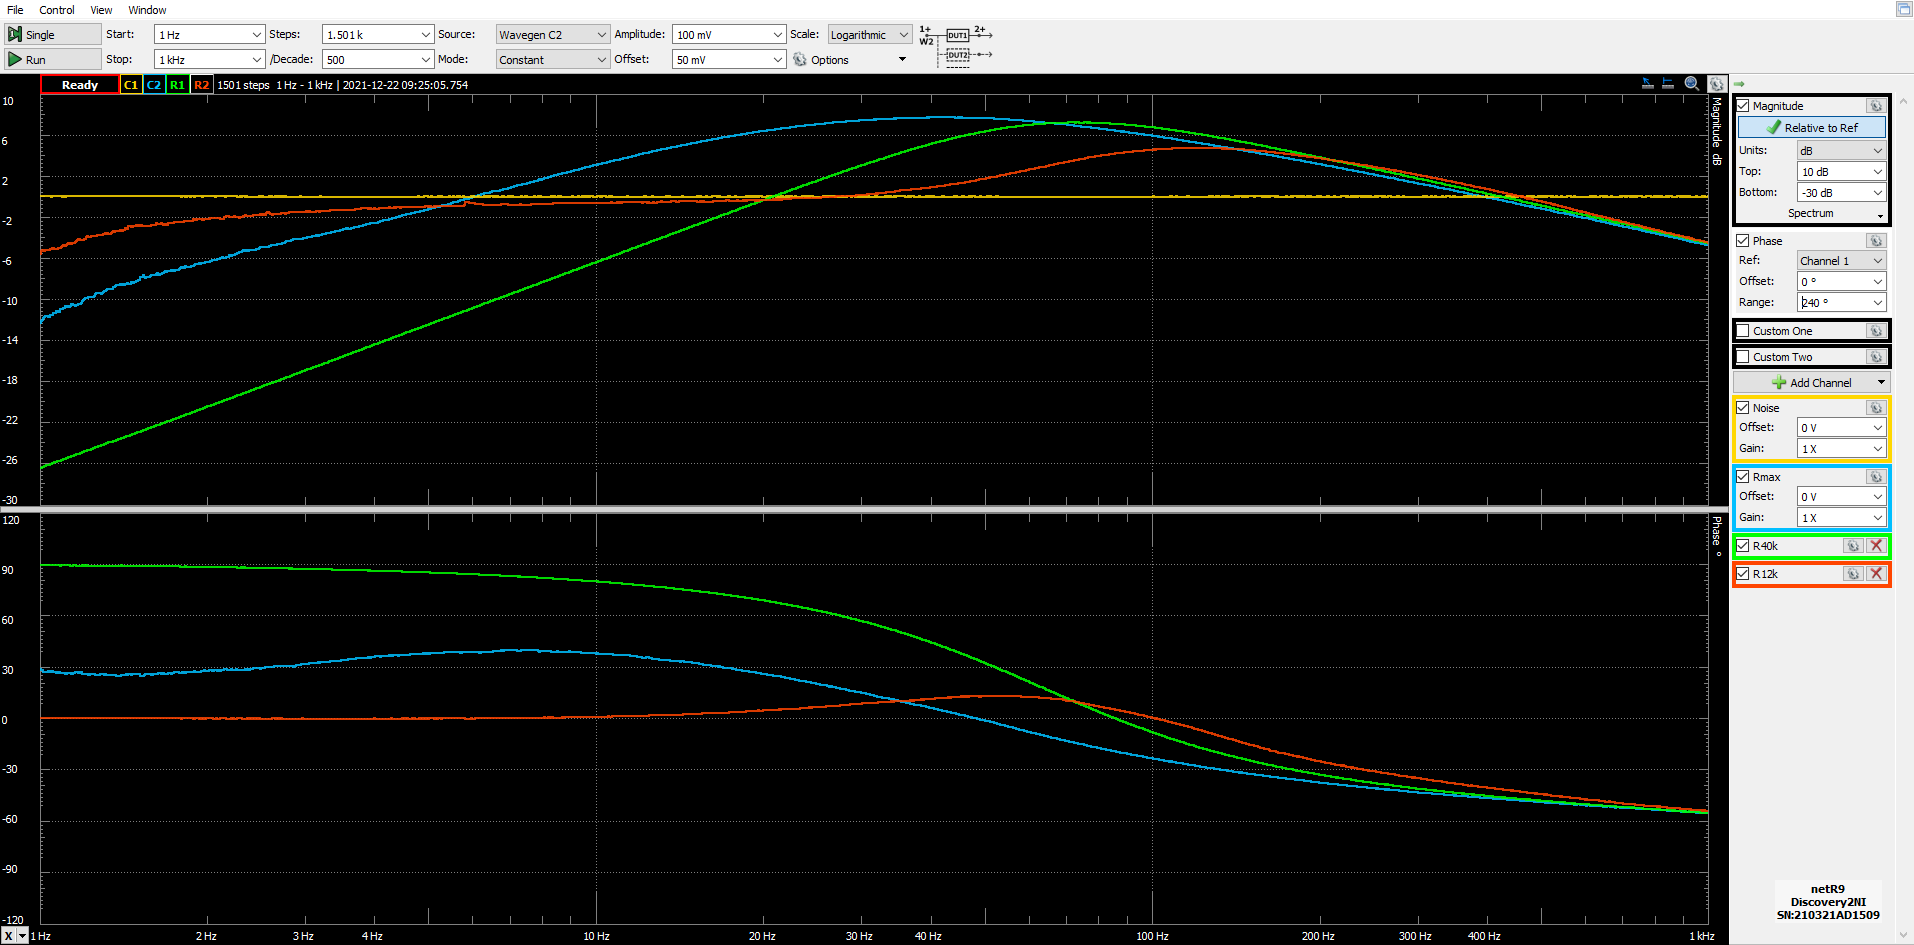
\includegraphics[width=\textwidth]{netR9func}
    \caption{Sovrapposizione dei plot di Bode ottenuti da scan di Network tra
    $\SI{1}{\Hz}$ e $\SI{1}{k\Hz}$ con un segnale sinusoidale in ingresso al
    LED di disturbo (ampiezza $v\ped{in} = \SI{100}{m\V}$, offset costante
    $\SI{50}{m\V}$) al variare della resistenza del potenziometro. 
	Rispettivamente in azzurro, verde e rosso la risposta in frequenza del
	segnale in \texttt{ERROR} per $R_9 = (103.0 \pm 0.6 \; \si{k\ohm})$,
	$(40.2 \pm 0.4 \; \si{k\ohm})$ e $(11.98 \pm 0.10 \; \si{k\ohm})$.
    \label{fig: netR9func}}
\end{figure}

Da cui si riesce a notare come la funzione di trasferimento abbia lo stesso
andamento asintotico per frequenze $f > \SI{1}{k\Hz}$, ma guadagno diverso
alle basse frequenze $f \sim 1 - 10 \; \si{\Hz}$ con cui si era disturbato in
precedenza. Questo risulta quindi compatibile con i risultati ottenuti nelle
sezioni precedenti e con l'andamento atteso del modulo della funzione di
trasferimento del controllore PI con un polo in $s = 0$, per cui\footnote{
indichiamo con $\tilde{f} (s)$ la trasformata di Laplace di $f(t)$, per cui
applicando il Teorema del valore finale}
\begin{equation}
V\ped{ERROR} (t = +\infty) = \lim_{s \to 0} s \tilde{V}\ped{ERROR}(s) = 0
\end{equation}
%Notiamo infine che dall'andamento trovato il prodotto banda-guadagno per
%gli amplificatori operazionali impiegati risulta almeno visivamente costante.

%=======================
\section*{Controllo proporzionale}
Infine si è costruito il circuito di controllo proporzionale a partire dal
precedente (integrale), scambiando il condensatore $C_1$ con una resistenza
$R_{10} = 100 \; \si{k\ohm}$ (nominali) secondo lo schema in \cref{schm: prop}.
\begin{figure}[htbp]
    \centering
	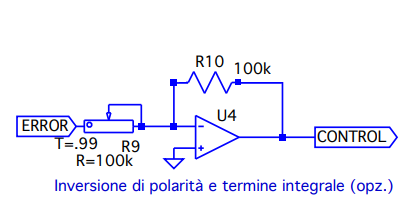
\includegraphics[scale=0.6]{controlgenprop}
    \caption{Schema circuitale del controllore ad azione proporzionale.
    \label{schm: prop}}
\end{figure}

Dunque ora il circuito completo non è altro che una cascata di
amplificatori, di cui il primo differenziale di guadagno nominale
$A_d = \frac{R_6}{R_5} = \frac{R_8}{R_7} = 10$, e il secondo invertente di
guadagno variabile in funzione della resistenza del potenziometro
$A_e = -\frac{R_{10}}{R_9}$.

Assumendo di poter descrivere la risposta complessiva del sensore di misura e
del controllore ad azione proporzionale di guadagno $K_p$ con una funzione di
trasferimento della forma
\begin{equation}
G(s) = \frac{A_0}{1 + 2\xi \tau s + \tau^2 s^2} \quad \text{con} \; \xi > 1
\end{equation}
Introducendo le notazioni più concise per i segnali di riferimento $r(t)$,
l'osservabile $y(t)$ e la loro differenza o errore $e(t) = r(t) - y(t)$
possiamo scrivere la trasformata di Laplace dell'errore come
\begin{equation}
\tilde{e}(s) = \frac{1}{s} \frac{1 + 2\xi \tau s + (\tau s)^2}
{1 + K_p A_0 + 2 \xi \tau s + (\tau s)^2}
\end{equation}
da cui è possibile vedere (al contrario del caso precedente) che il
controllore ad azione proporzionale non riesce ad annullare l'errore neanche
a regime, infatti dal teorema del valore finale abbiamo:
\begin{equation}\label{eq: Pfv}
e (t = +\infty) = \lim_{s \to 0} s \tilde{e}(s) = \frac{1}{1 + K_p A_0}
\end{equation}
che tende a 0 al crescere di $K_p$ soltanto nel limite in cui $K_p A_0 \gg 1$.

\section{Risposta ad un'onda quadra}
Esattamente come all'inizio della \cref{sec: intsqwresp} si è reimpostato
il potenziometro $R_9$ fino alla sua massima resistenza e si è pilotato il
driver LED di disturbo con un'onda quadra compresa tra $0$ e
$150 \; \si{m\V}$ con frequenza fissata a $f = 1 \si{\Hz}$.

Dunque si è studiata nuovamente la risposta del circuito osservando
l'andamento temporale dei segnali nelle uscite \verb+ERROR+, \verb+CONTROL+ e
\verb+MEAS+.
\begin{figure}[htbp]
    \centering
	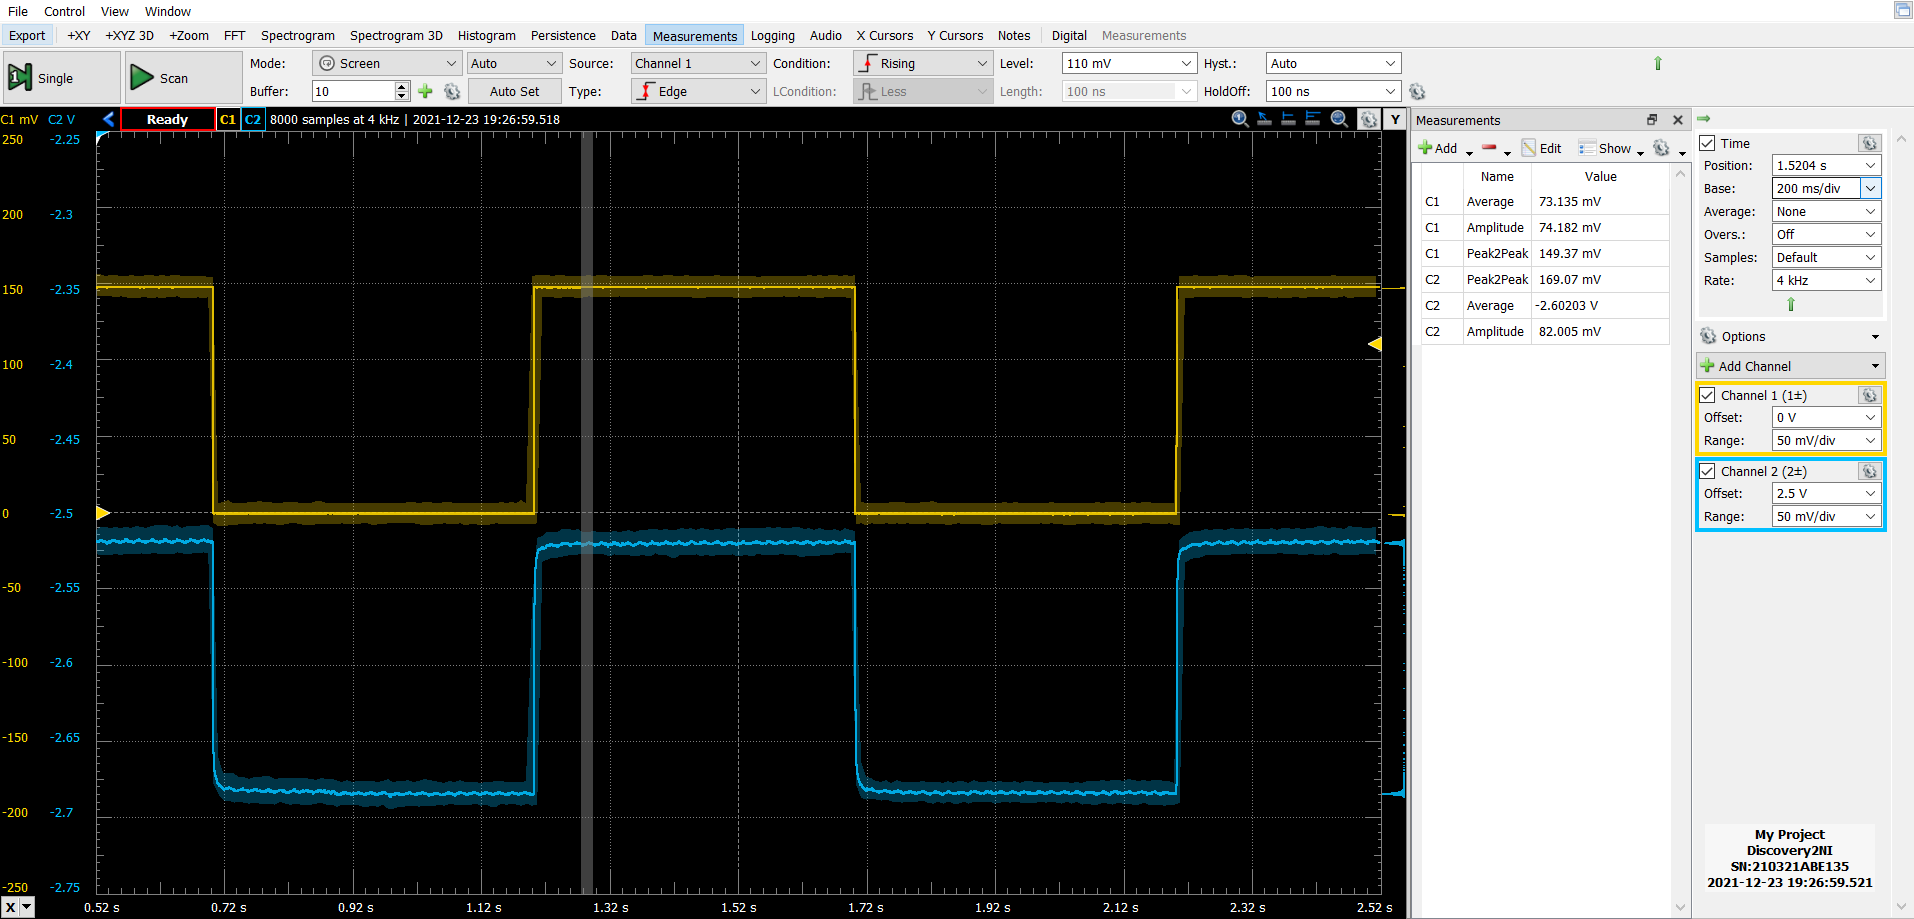
\includegraphics[width=\textwidth]{proportional}
    \caption{Acquisizione presa dall'oscilloscopio dei segnali
    $V\ped{ERROR}(t)$ (CH1) e dell'onda pilota di disturbo $W_2 (t)$ (CH2).
    \label{fig: properrnoise}}
\end{figure}
\begin{figure}[htbp]
    \centering
	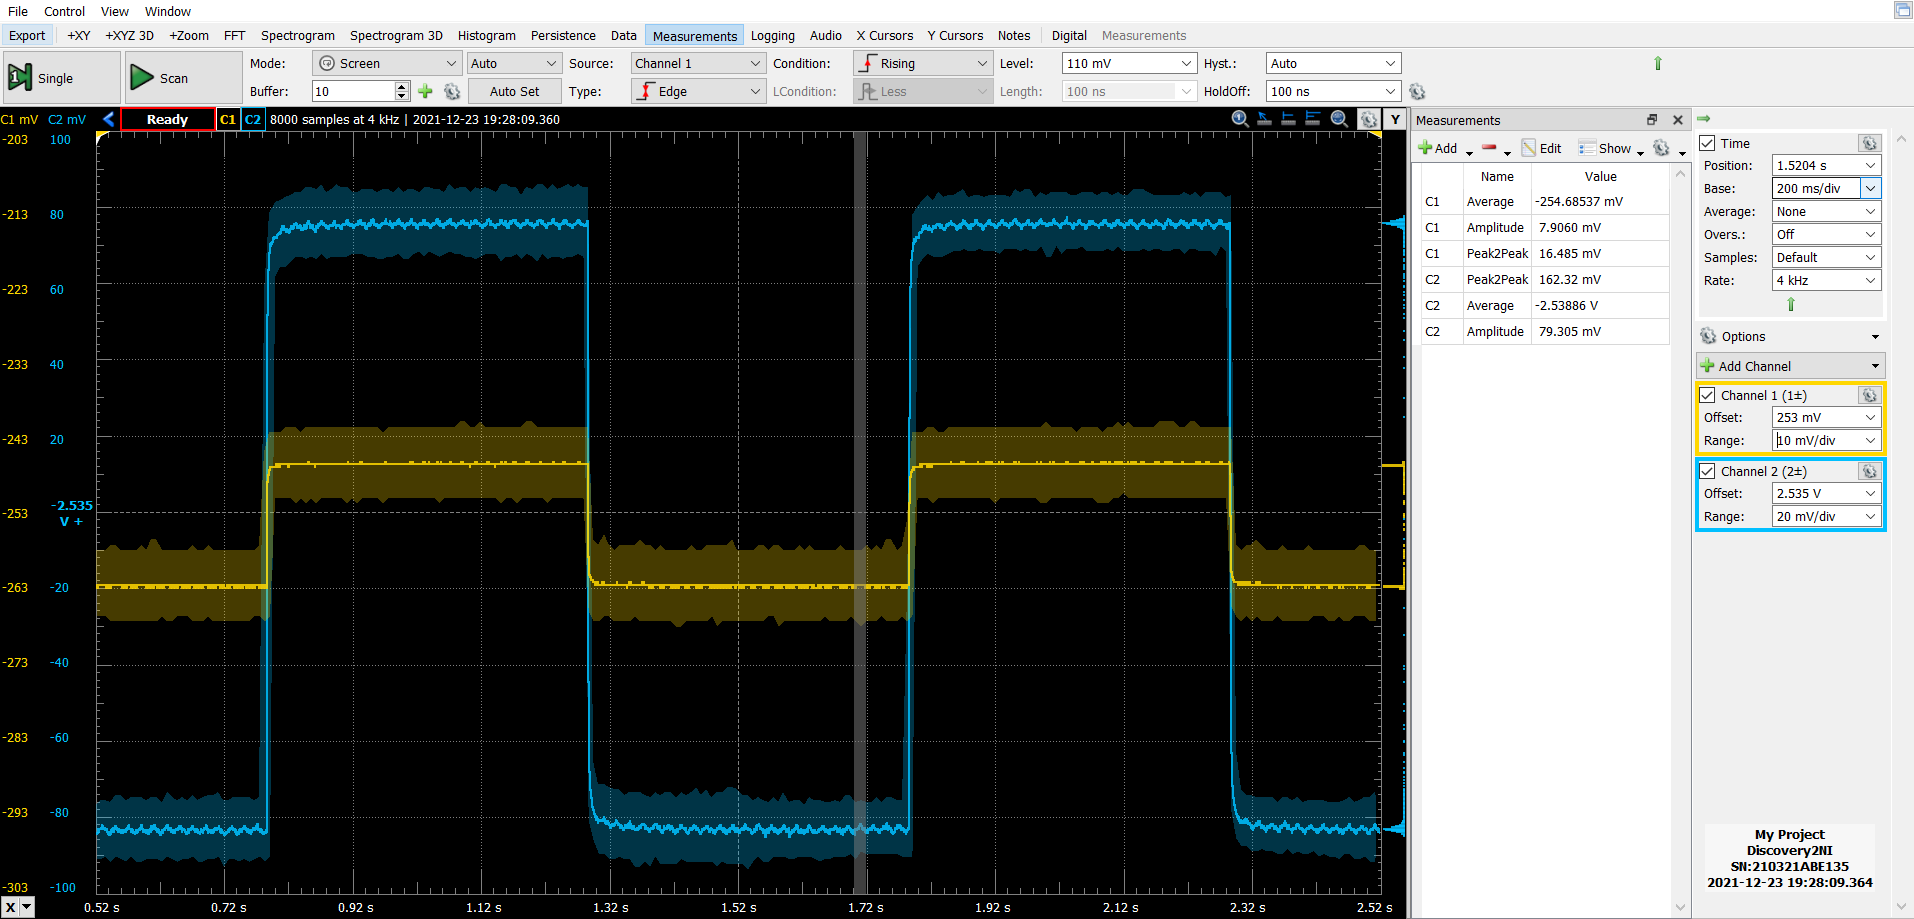
\includegraphics[width=\textwidth]{proportional.meas}
    \caption{Acquisizione dell'andamento nel tempo dei segnali in
    \texttt{ERROR} (CH1) e di \texttt{MEAS} misurato rispetto a \texttt{SET}
    (CH2).
    \label{fig: properrmeas}}
\end{figure}
\begin{figure}[htbp]
    \centering
	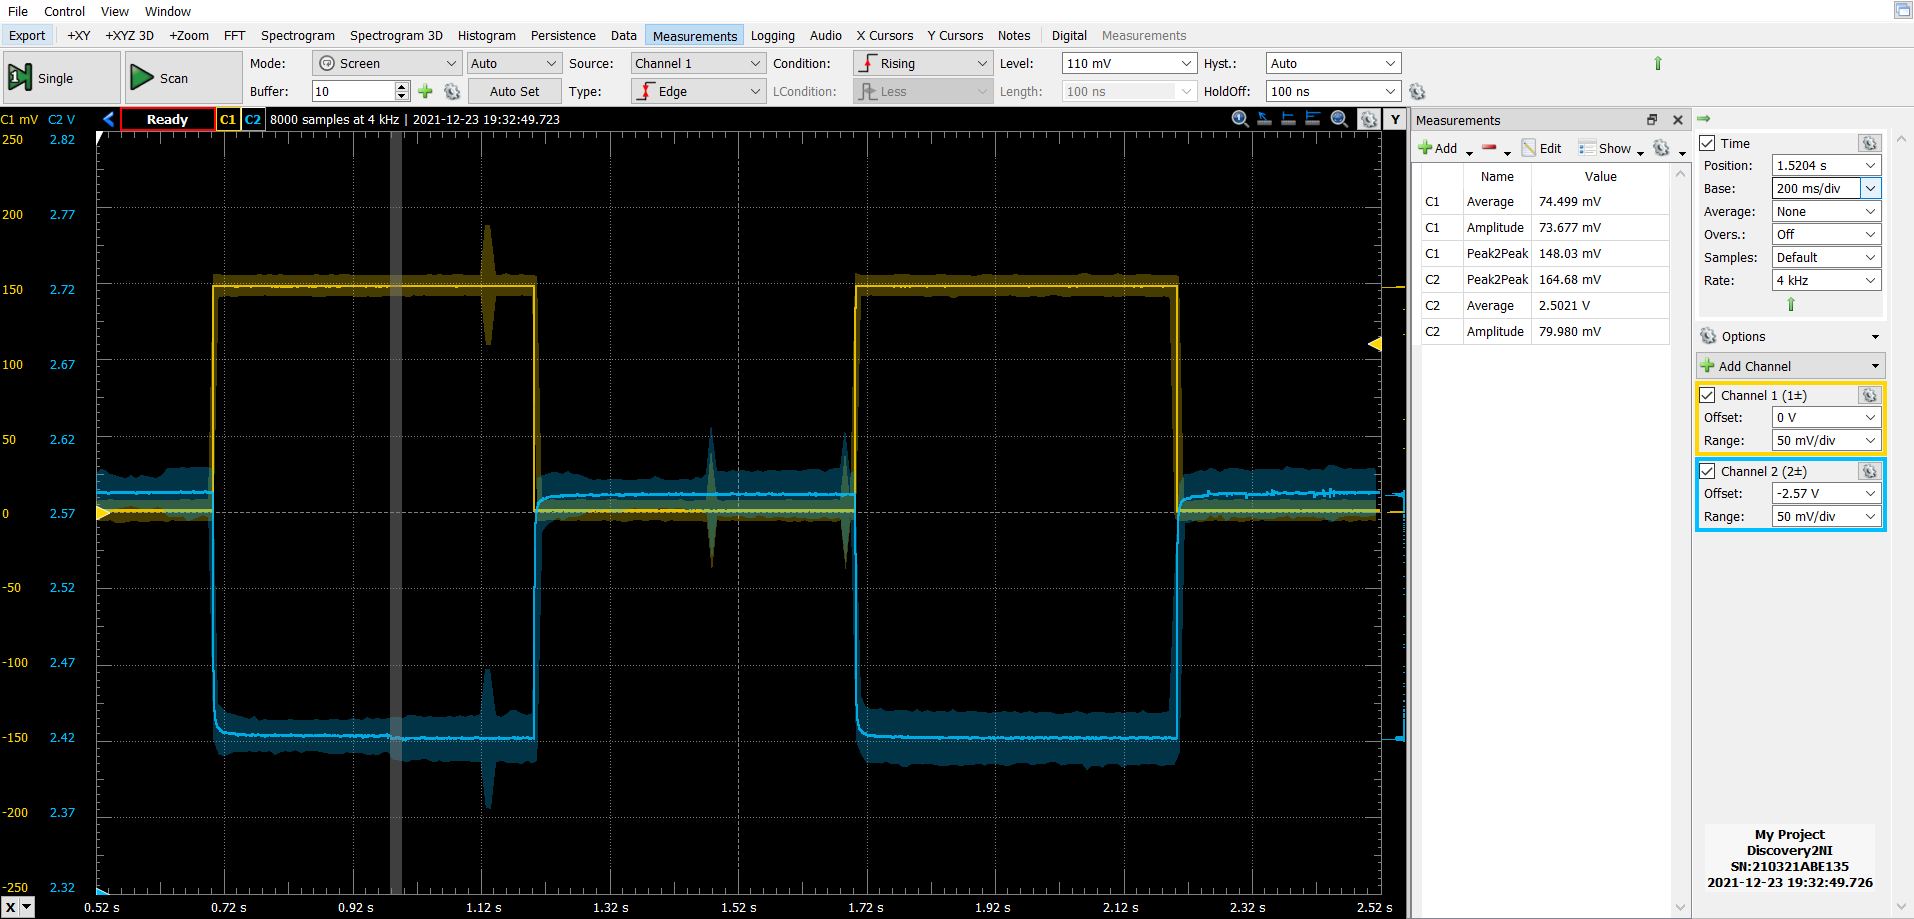
\includegraphics[width=\textwidth]{proportional.control}
    \caption{Acquisizione presa dall'oscilloscopio dei segnali
    $V\ped{CONTROL} (t)$ (CH1) e dell'onda pilota del LED di disturbo
    $W_2 (t)$ (CH2).
    \label{fig: propctrlnoise}}
\end{figure}

Per mostrare come si modifica la risposta del segnale $V\ped{ERROR} (t)$ al
variare della resistenza $R_9$ si riportano in un unico grafico varie
acquisizioni del suo andamento nel tempo osservate all'oscilloscopio 
in \cref{fig: propR9}.
\begin{figure}[htbp]
    \centering
	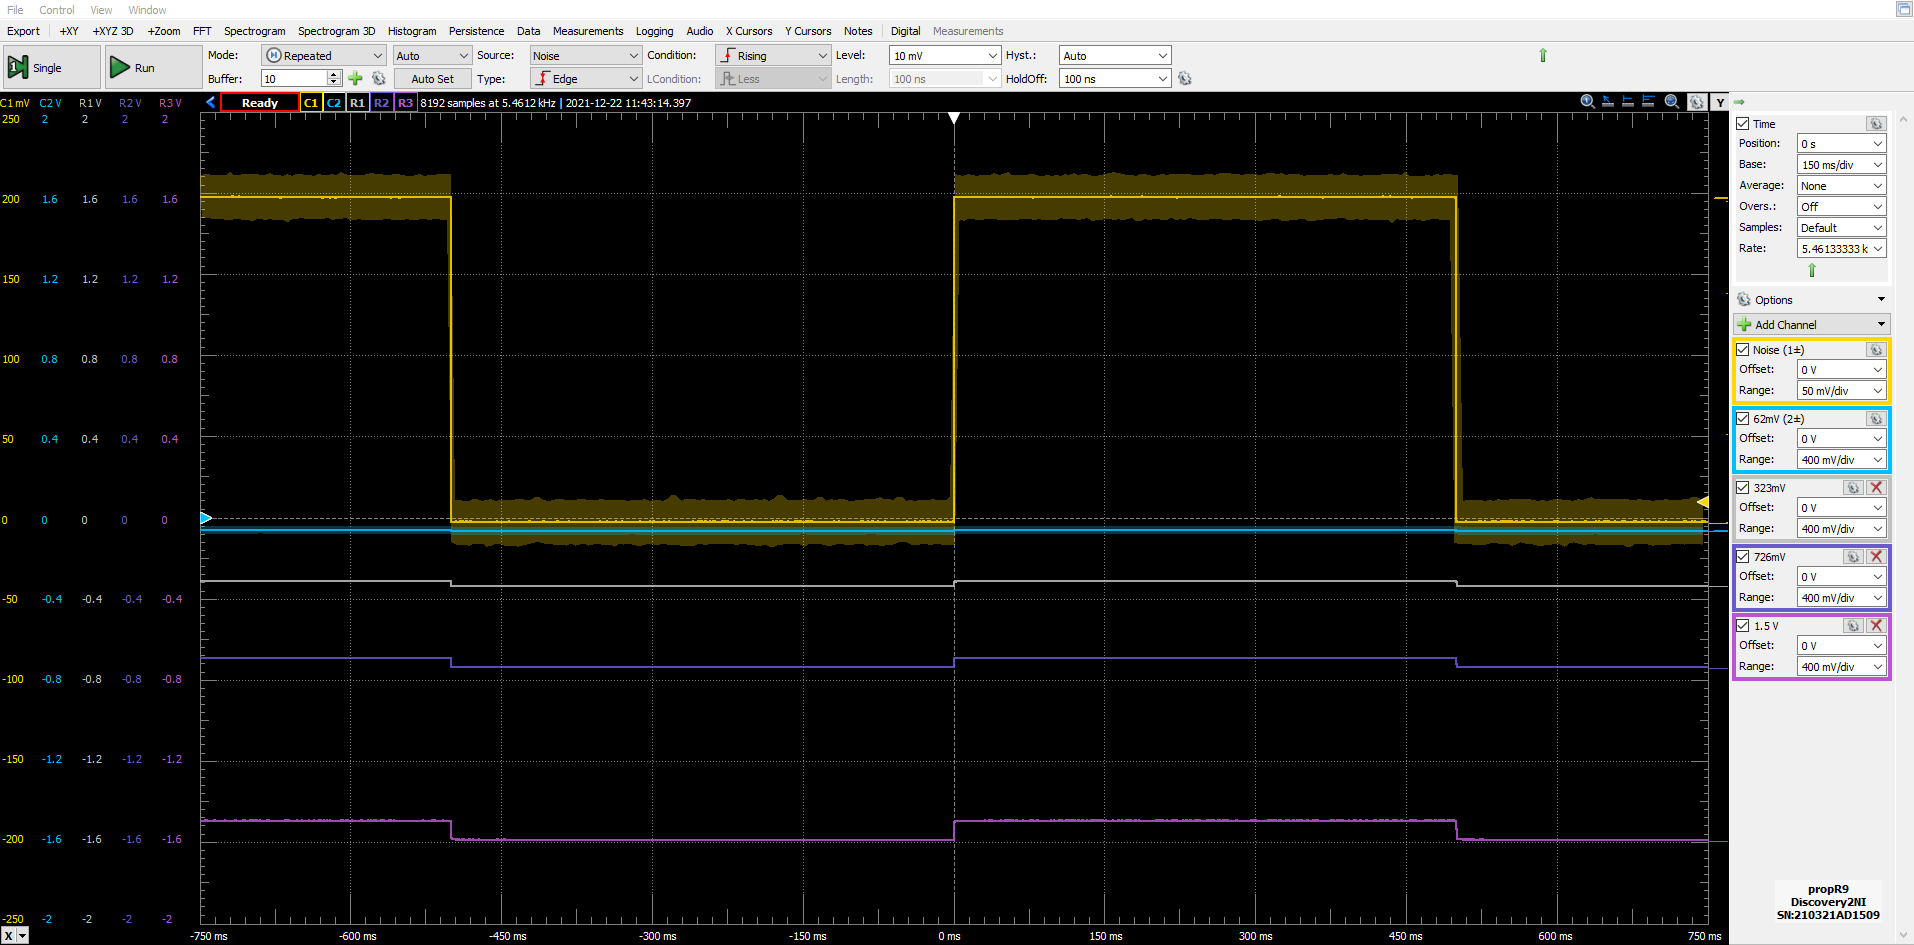
\includegraphics[width=\textwidth]{propR9}
    \caption{Acquisizione all'oscilloscopio della modifica del segnale
    $V\ped{ERROR} (t)$ (CH2) al diminuire della resistenza del potenziometro
    $R_9$. Dal basso verso l'alto in ordine di offset decrescente (in modulo)
    per $R_9 \approx (60 \; \si{k\ohm})$, $(40 \si{k\ohm})$,
    $(12 \; \si{k\ohm})$, $(3 \; \si{k\ohm})$.
    In giallo l'onda quadra di disturbo $W_2 (t)$ su (CH1).
    \label{fig: propR9}}
\end{figure}

Da cui notiamo che il segnale d'errore ha la forma di un'onda quadra in
opposizione di fase a quella in \verb+NOISE+ di ampiezza e offset decrescenti
al diminuire della resistenza $R_9$, ma che per nessun valore di questa arriva
al livello $0$ V. Questo risulta compatibile con la risposta attesa per
l'offset osservato in \verb+ERROR+ dalla \cref{eq: Pfv} in conseguenza
dell'aumento di $K_p \propto A_e$ dovuto alla riduzione del valore di
resistenza $R_9$.

%=======================
\section*{Conclusioni e commenti finali}
Si è riusciti a costruire e studiare un circuito controllore ad azione
proporzionale/integrale di luminosità ambientale basato sulla lettura di una
foto-resistenza.

In particolare siamo riusciti a descrivere e verificarne sperimentalmente il
funzionamento e a caratterizzarne la risposta al variare dei parametri di
costruzione del circuito e delle fonti di disturbo nel dominio dei tempi e
delle frequenze.

%=======================
\section*{Dichiarazione}
I firmatari di questa relazione dichiarano che il contenuto della relazione \`e
originale, con misure effettuate dai membri del gruppo, e che tutti i firmatari
hanno contribuito alla elaborazione della relazione stessa.
\end{document}
